% Sgr A* Scientific Simulator — EXTENSION paper (plan gates G13–G24).
% A separate document: it is NOT \input into ../thesis.tex. Same class and
% layout as the thesis. Compile: make -C paper extension (pdflatex ×3 +
% bibtex). numbers_ext.tex, tab_*.tex and figures/ are auto-generated by
% `make reproduce-ext`; every quantitative statement that is not a cited
% literature value comes from a \newcommand there.
\documentclass[12pt,a4paper]{report}

\usepackage[a4paper,margin=3.2cm]{geometry}
\linespread{1.27}
\usepackage{amsmath}
\usepackage{amssymb}
\usepackage{graphicx}
\usepackage{booktabs}
\usepackage{longtable}
\usepackage[round]{natbib}
\usepackage[hidelinks]{hyperref}

\setcounter{tocdepth}{2}
\setcounter{secnumdepth}{2}

\makeatletter
\def\verbatim@font{\normalfont\ttfamily\small}
\makeatother

% Numbers: the thesis' (shared calibration constants) and this paper's own.
% AUTO-GENERATED by scripts/make_numbers.py — do not edit by hand.
% Regenerate with `make reproduce` / `py -3.11 scripts/make_numbers.py`.
\newcommand{\FitMass}{4.270}
\newcommand{\FitMassErr}{0.195}
\newcommand{\FitDist}{8272}
\newcommand{\FitDistErr}{182}
\newcommand{\FitSma}{124.82}
\newcommand{\FitSmaErr}{0.88}
\newcommand{\FitEcc}{0.88277}
\newcommand{\FitEccErr}{0.00195}
\newcommand{\FitIncl}{134.70}
\newcommand{\FitInclErr}{0.41}
\newcommand{\FitOmegaBig}{227.33}
\newcommand{\FitOmegaBigErr}{0.63}
\newcommand{\FitOmegaSm}{65.44}
\newcommand{\FitOmegaSmErr}{0.61}
\newcommand{\FitTPeri}{2002.3227}
\newcommand{\FitTPeriErr}{0.0052}
\newcommand{\FitPeriod}{16.0561}
\newcommand{\FitPeriodErr}{0.0228}
\newcommand{\FitChiTwo}{307.8}
\newcommand{\FitDof}{321}
\newcommand{\FitChiRed}{0.959}
\newcommand{\FitNAst}{145}
\newcommand{\FitNRv}{44}
\newcommand{\GrExcessPeak}{205}
\newcommand{\GrExcessEpoch}{2018.379}
\newcommand{\PrecSchw}{11.98}
\newcommand{\PrecLT}{-0.204}
\newcommand{\FitMassNSigma}{0.14}
\newcommand{\FitDistNSigma}{0.03}
\newcommand{\EpsQBest}{0.00}
\newcommand{\EpsQSigma}{0.93}
\newcommand{\EpsQCiNinetyFive}{1.33}
\newcommand{\EpsQForecastTenOrbits}{0.34}
\newcommand{\SchwDiamM}{10.3924}
\newcommand{\SchwSpreadPct}{0.000}
\newcommand{\KerrDiamM}{9.5445}
\newcommand{\KerrDiamUas}{48.91}
\newcommand{\BeamRatio}{9.60}
\newcommand{\GMin}{0.139}
\newcommand{\GMax}{1.440}
\newcommand{\FluxRatioZeroOne}{10.7}
\newcommand{\FluxRatioOneTwo}{274}
\newcommand{\CalDiamUas}{49.68}
\newcommand{\CalDiamM}{9.695}
\newcommand{\CalAxisRatio}{0.9946}
\newcommand{\UasPerM}{5.1243}
\newcommand{\GpuMeanDiff}{0.00289}
\newcommand{\GpuMaxDiff}{0.697}
\newcommand{\GpuOutliers}{32}
\newcommand{\BenchCpuNullStepsPerS}{1,340,753}
\newcommand{\BenchCpuChristoffelPerS}{508,369}
\newcommand{\BenchCpuTimelikeStepsPerS}{78,987}
\newcommand{\BenchGpuFpsHd}{47.5}
\newcommand{\BenchGpuFpsFullhd}{21}
\newcommand{\BenchGpuMegaraysPerSHd}{43.8}
\newcommand{\EtaSchw}{5.72}
\newcommand{\EtaSgrA}{17.96}
\newcommand{\EtaNearExtremal}{32.10}
\newcommand{\GammaPolarSgrA}{2.571}
\newcommand{\GammaProSgrA}{3.142}
\newcommand{\GammaRetroSgrA}{3.142}
\newcommand{\ProjOnWorstDev}{9.6\times10^{-12}}
\newcommand{\ProjOffWorstPct}{93}
\newcommand{\ProjOffBestDev}{1.1\times10^{-04}}
\newcommand{\SubringRatioZeroOneLo}{8.6}
\newcommand{\SubringRatioZeroOneHi}{16.8}

% AUTO-GENERATED by scripts/make_numbers_ext.py — do not edit by hand.
% Regenerate with `make reproduce-ext`.
\newcommand{\XLiveNpix}{24\,728}
\newcommand{\XLiveDlnYMed}{0.000}
\newcommand{\XLiveDlnYPninetyfive}{2.0}
\newcommand{\XLiveChromaMed}{0.000}
\newcommand{\XLiveBeamCpu}{17.9}
\newcommand{\XLiveBeamGpu}{18.0}
\newcommand{\XLiveBeamErr}{0.26}
\newcommand{\XLiveMaskMismatch}{0.33}
\newcommand{\XLiveTpeak}{6\,300}
\newcommand{\XEta}{0.181}
\newcommand{\XRisco}{2.024}
\newcommand{\XMdotLow}{2\times10^{-9}}
\newcommand{\XTpeakLow}{7\,280}
\newcommand{\XLumLow}{2.1\times10^{37}}
\newcommand{\XLumEddLow}{3.8\times10^{-8}}
\newcommand{\XLumFactorLow}{12}
\newcommand{\XChromXLow}{0.303}
\newcommand{\XChromYLow}{0.313}
\newcommand{\XMdotMid}{2\times10^{-8}}
\newcommand{\XTpeakMid}{12\,900}
\newcommand{\XLumMid}{2.1\times10^{38}}
\newcommand{\XLumEddMid}{3.8\times10^{-7}}
\newcommand{\XLumFactorMid}{120}
\newcommand{\XChromXMid}{0.269}
\newcommand{\XChromYMid}{0.274}
\newcommand{\XMdotHigh}{2\times10^{-7}}
\newcommand{\XTpeakHigh}{23\,000}
\newcommand{\XLumHigh}{2.1\times10^{39}}
\newcommand{\XLumEddHigh}{3.8\times10^{-6}}
\newcommand{\XLumFactorHigh}{1\,200}
\newcommand{\XChromXHigh}{0.254}
\newcommand{\XChromYHigh}{0.254}
\newcommand{\XRpeak}{2.95}
\newcommand{\XLEdd}{5.4\times10^{44}}
\newcommand{\XGmax}{1.309}
\newcommand{\XGmin}{0.168}
\newcommand{\XBoloContrast}{52.2}
\newcommand{\XVisContrastRef}{1\,090}
\newcommand{\XVisContrastLow}{438}
\newcommand{\XVisContrastMid}{35.3}
\newcommand{\XVisContrastHigh}{9.60}
\newcommand{\XContrastCrossT}{11\,500}
\newcommand{\XVisBoloRatio}{21}
\newcommand{\XAppChromX}{0.293}
\newcommand{\XAppChromY}{0.302}
\newcommand{\XRecChromX}{0.635}
\newcommand{\XRecChromY}{0.361}
\newcommand{\XSyngeDeg}{27.69}
\newcommand{\XInfallEdgeDeg}{17.32}
\newcommand{\XInfallSpeedTen}{0.4472}
\newcommand{\XOrbitSpeedTen}{0.3536}
\newcommand{\XOrbitEdgeRightDeg}{44.65}
\newcommand{\XOrbitEdgeLeftDeg}{7.65}
\newcommand{\XAberrationCheck}{2\times10^{-12}}
\newcommand{\XInfallSpeedHorizon}{0.99989}
\newcommand{\XRplus}{1.3412}
\newcommand{\XRphPro}{1.43}
\newcommand{\XRphRetro}{3.95}
\newcommand{\XRergoEq}{2}
\newcommand{\XIscoSpeedSchw}{0.5000}
\newcommand{\XIscoClockSchw}{0.7071}
\newcommand{\XHoverSpeedSix}{0.0628}
\newcommand{\XKerrZamoLeftDeg}{13.66}
\newcommand{\XKerrZamoRightDeg}{37.32}
\newcommand{\XKerrOrbitLeftDeg}{5.47}
\newcommand{\XKerrOrbitRightDeg}{51.04}
\newcommand{\XObsGpuMaxPx}{0.72}
\newcommand{\XObsGpuCases}{14}
\newcommand{\XObsGpuPixel}{0.00140}
\newcommand{\XLegacyBudgetPx}{16.8}
\newcommand{\XLegacyBudgetSteps}{1600}
\newcommand{\XBudgetSteps}{6000}
\newcommand{\XMinPerM}{0.3527}
\newcommand{\XRPforty}{6.64}
\newcommand{\XFlGraR}{7.00}
\newcommand{\XFlGraIncl}{160}
\newcommand{\XFlGraPeriod}{43.1}
\newcommand{\XFlGraPeriodM}{122.3}
\newcommand{\XFlGraLoop}{74.4}
\newcommand{\XFlGraOrbit}{71.7}
\newcommand{\XFlGraChord}{64}
\newcommand{\XFlGraChordSpeed}{0.15}
\newcommand{\XFlGraPathSpeed}{0.36}
\newcommand{\XFlGraContrast}{2.23}
\newcommand{\XFlGraContrastSix}{2.60}
\newcommand{\XFlGraLensed}{6.5}
\newcommand{\XFlGraEchoMin}{16.8}
\newcommand{\XFlGraEchoMax}{25.8}
\newcommand{\XFlGraEchoMean}{21.4}
\newcommand{\XFlGraEchoMeanMin}{7.5}
\newcommand{\XFlGraEchoMinMin}{5.9}
\newcommand{\XFlGraEchoMaxMin}{9.1}
\newcommand{\XFlGraOffset}{2.1}
\newcommand{\XFlGraEchoPeakMin}{2.8}
\newcommand{\XFlGraEchoPeakMax}{11.4}
\newcommand{\XFlGraNoiseFlux}{0.22}
\newcommand{\XFlGraNoiseCentroid}{0.16}
\newcommand{\XFlGraSense}{clockwise}
\newcommand{\XFlGrbR}{9.00}
\newcommand{\XFlGrbIncl}{140}
\newcommand{\XFlGrbPeriod}{61.9}
\newcommand{\XFlGrbPeriodM}{175.6}
\newcommand{\XFlGrbLoop}{96.6}
\newcommand{\XFlGrbOrbit}{92.2}
\newcommand{\XFlGrbChord}{97}
\newcommand{\XFlGrbChordSpeed}{0.22}
\newcommand{\XFlGrbPathSpeed}{0.30}
\newcommand{\XFlGrbContrast}{3.92}
\newcommand{\XFlGrbContrastSix}{5.11}
\newcommand{\XFlGrbLensed}{4.1}
\newcommand{\XFlGrbEchoMin}{13.3}
\newcommand{\XFlGrbEchoMax}{47.0}
\newcommand{\XFlGrbEchoMean}{28.6}
\newcommand{\XFlGrbEchoMeanMin}{10.1}
\newcommand{\XFlGrbEchoMinMin}{4.7}
\newcommand{\XFlGrbEchoMaxMin}{16.6}
\newcommand{\XFlGrbOffset}{4.9}
\newcommand{\XFlGrbEchoPeakMin}{0.1}
\newcommand{\XFlGrbEchoPeakMax}{16.4}
\newcommand{\XFlGrbNoiseFlux}{0.31}
\newcommand{\XFlGrbNoiseCentroid}{0.39}
\newcommand{\XFlGrbSense}{clockwise}
\newcommand{\XFlPfoR}{6.64}
\newcommand{\XFlPfoIncl}{160}
\newcommand{\XFlPfoPeriod}{40.0}
\newcommand{\XFlPfoPeriodM}{113.4}
\newcommand{\XFlPfoLoop}{70.5}
\newcommand{\XFlPfoOrbit}{68.0}
\newcommand{\XFlPfoChord}{54}
\newcommand{\XFlPfoChordSpeed}{0.12}
\newcommand{\XFlPfoPathSpeed}{0.37}
\newcommand{\XFlPfoContrast}{2.27}
\newcommand{\XFlPfoContrastSix}{2.65}
\newcommand{\XFlPfoLensed}{7.1}
\newcommand{\XFlPfoEchoMin}{16.4}
\newcommand{\XFlPfoEchoMax}{25.2}
\newcommand{\XFlPfoEchoMean}{20.9}
\newcommand{\XFlPfoEchoMeanMin}{7.4}
\newcommand{\XFlPfoEchoMinMin}{5.8}
\newcommand{\XFlPfoEchoMaxMin}{8.9}
\newcommand{\XFlPfoOffset}{2.0}
\newcommand{\XFlPfoEchoPeakMin}{2.9}
\newcommand{\XFlPfoEchoPeakMax}{12.3}
\newcommand{\XFlPfoNoiseFlux}{0.22}
\newcommand{\XFlPfoNoiseCentroid}{0.15}
\newcommand{\XFlPfoSense}{clockwise}
\newcommand{\XFlPixels}{256}
\newcommand{\XFlHalfWidth}{14}
\newcommand{\XFlSigma}{0.5}
\newcommand{\XFlMaxdH}{5\times10^{-10}}
\newcommand{\XFlMaxdL}{1\times10^{-10}}
\newcommand{\XFlResHalf}{128}
\newcommand{\XFlResLoop}{1.7}
\newcommand{\XFlResContrast}{3.0}
\newcommand{\XFlResEcho}{0.6}
\newcommand{\XFlResChord}{0.9}
\newcommand{\XFlGpuFluxDev}{0.6}
\newcommand{\XFlGpuCentroidPx}{0.27}
\newcommand{\XFlGpuCorr}{0.992}
\newcommand{\XRiafTarget}{2.4}
\newcommand{\XRiafBeam}{20}
\newcommand{\XRiafNzero}{2.7\times10^{7}}
\newcommand{\XRiafFlux}{2.40}
\newcommand{\XRiafTzero}{1.5\times10^{11}}
\newcommand{\XRiafBeta}{10}
\newcommand{\XRiafPixels}{160}
\newcommand{\XRiafHalfWidth}{12}
\newcommand{\XRiafDraw}{42.8}
\newcommand{\XRiafRingDeficit}{17}
\newcommand{\XRiafAraw}{0.43}
\newcommand{\XRiafDblur}{25.3}
\newcommand{\XRiafWdBlur}{1.15}
\newcommand{\XRiafAblur}{0.33}
\newcommand{\XRiafNullMin}{3.90}
\newcommand{\XRiafNullMax}{9.95}
\newcommand{\XRiafNullPAs}{26}
\newcommand{\XRiafThinRing}{40.5}
\newcommand{\XRiafTb}{4.2\times10^{10}}
\newcommand{\XRiafTbBlur}{3.2\times10^{10}}
\newcommand{\XRiafTeIsco}{8.3\times10^{10}}
\newcommand{\XRiafBIsco}{62}
\newcommand{\XRiafNeIsco}{1.2\times10^{7}}
\newcommand{\XRiafMaxdH}{3\times10^{-9}}
\newcommand{\XRiafResD}{0.7}
\newcommand{\XRiafResLow}{120}
\newcommand{\XRiafHalfNull}{3.20}
\newcommand{\XRiafHalfThin}{49}
\newcommand{\XRiafHalfA}{0.08}
\newcommand{\XRiafTenD}{49.2}
\newcommand{\XPolPzero}{0.7}
\newcommand{\XPolTorArg}{1}
\newcommand{\XPolRadArgCw}{+168}
\newcommand{\XPolRadArgCcw}{-168}
\newcommand{\XPolVerArgCcw}{+135}
\newcommand{\XPolVerArgCw}{-135}
\newcommand{\XPolVerRatio}{0.8}
\newcommand{\XPolVerBetaTwo}{0.27}
\newcommand{\XPolVerM}{42}
\newcommand{\XRiafGpuFluxDev}{0.2}
\newcommand{\XRiafGpuCorr}{0.9999}
\newcommand{\XRiafGpuCentroidPx}{0.03}
\newcommand{\XWhA}{0.01}
\newcommand{\XWhW}{0.05}
\newcommand{\XWhWoverM}{1.42953}
\newcommand{\XWhM}{0.03498}
\newcommand{\XWhWdiff}{9\times10^{-16}}
\newcommand{\XWhRTwo}{2.834}
\newcommand{\XWhEdgeTwo}{20.659}
\newcommand{\XWhRingTwo}{21.662}
\newcommand{\XWhRSix}{6.796}
\newcommand{\XWhEdgeSix}{8.462}
\newcommand{\XWhRingSix}{10.120}
\newcommand{\XWhRFifteen}{15.764}
\newcommand{\XWhEdgeFifteen}{3.637}
\newcommand{\XWhRingFifteen}{5.428}
\newcommand{\XWhEdgeErr}{7\times10^{-12}}
\newcommand{\XWhMaxdB}{4\times10^{-16}}
\newcommand{\XWhMaxH}{7\times10^{-12}}
\newcommand{\XWhRingShift}{3\times10^{-6}}
\newcommand{\XWhGpuMaxPx}{0.28}
\newcommand{\XWhGpuStrip}{2001}
\newcommand{\XFcGravAst}{65}
\newcommand{\XFcGravRate}{18}
\newcommand{\XFcGravRv}{12}
\newcommand{\XFcGravRvRate}{5}
\newcommand{\XFcExAst}{0.4}
\newcommand{\XFcExRate}{9.2}
\newcommand{\XFcExRv}{45}
\newcommand{\XFcExRvRate}{2.7}
\newcommand{\XFcPlummer}{0.3}
\newcommand{\XFcApo}{0.235}
\newcommand{\XFcEncl}{23.5}
\newcommand{\XFcPeriod}{16.06}
\newcommand{\XFcGspan}{24.3}
\newcommand{\XFcGnAst}{145}
\newcommand{\XFcGnRv}{44}
\newcommand{\XFcSigEpsFisher}{93\,500}
\newcommand{\XFcSigEpsThesis}{93\,500}
\newcommand{\XFcSigEpsDiff}{0.0}
\newcommand{\XFcSigMDiff}{0.09}
\newcommand{\XFcTenFisher}{577}
\newcommand{\XFcTenThesis}{34\,000}
\newcommand{\XFcTenGain}{162}
\newcommand{\XFcTenGainThesis}{2.8}
\newcommand{\XFcEpsGravEight}{5\,600}
\newcommand{\XFcEpsExEight}{19\,000}
\newcommand{\XFcEpsGravSixteen}{3\,700}
\newcommand{\XFcEpsExSixteen}{10\,000}
\newcommand{\XFcEpsGravThirtyTwo}{840}
\newcommand{\XFcEpsExThirtyTwo}{4\,800}
\newcommand{\XFcEpsGravSixtyFour}{290}
\newcommand{\XFcEpsExSixtyFour}{2\,000}
\newcommand{\XFcLtThreeSixtyFive}{114}
\newcommand{\XFcLtFiveSixtyFive}{\ensuremath{>160}}
\newcommand{\XFcLtThreeThirty}{70}
\newcommand{\XFcLtFiveThirty}{98}
\newcommand{\XFcLtThreeTen}{34}
\newcommand{\XFcLtFiveTen}{50}
\newcommand{\XFcLtThreeSixtyFiveMarg}{\ensuremath{>160}}
\newcommand{\XFcLtFiveSixtyFiveMarg}{\ensuremath{>160}}
\newcommand{\XFcLtThreeThirtyMarg}{160}
\newcommand{\XFcLtFiveThirtyMarg}{\ensuremath{>160}}
\newcommand{\XFcLtThreeTenMarg}{77}
\newcommand{\XFcLtFiveTenMarg}{108}
\newcommand{\XFcStepCheck}{2.3}
\newcommand{\XFcNrowsEight}{662}
\newcommand{\XFcChiScatterEight}{36}
\newcommand{\XFcNrowsSixteen}{990}
\newcommand{\XFcChiScatterSixteen}{44}
\newcommand{\XFcNrowsThirtyTwo}{1646}
\newcommand{\XFcChiScatterThirtyTwo}{57}
\newcommand{\XFcCorrGs}{-0.79}
\newcommand{\XFcSigEncGs}{0.854}
\newcommand{\XFcSigEncMargGs}{1.379}
\newcommand{\XFcInflGs}{1.61}
\newcommand{\XFcCorrEight}{-0.45}
\newcommand{\XFcSigEncEight}{0.076}
\newcommand{\XFcSigEncMargEight}{0.085}
\newcommand{\XFcInflEight}{1.12}
\newcommand{\XFcCorrSixteen}{-0.60}
\newcommand{\XFcSigEncSixteen}{0.043}
\newcommand{\XFcSigEncMargSixteen}{0.054}
\newcommand{\XFcInflSixteen}{1.25}
\newcommand{\XFcCorrThirtyTwo}{-0.58}
\newcommand{\XFcSigEncThirtyTwo}{0.012}
\newcommand{\XFcSigEncMargThirtyTwo}{0.014}
\newcommand{\XFcInflThirtyTwo}{1.23}
\newcommand{\XFcProfAgree}{8}
\newcommand{\XFcBiasEpsHalfThirtyTwo}{2.5}
\newcommand{\XFcBiasEpsGs}{0.1}
\newcommand{\XFcBiasMGs}{+0.05}
\newcommand{\XFcChiLeftGs}{0.014}
\newcommand{\XFcChiSignalGs}{44}
\newcommand{\XFcBiasLinRatioGs}{1.26}
\newcommand{\XFcBiasEpsEight}{0.5}
\newcommand{\XFcBiasMEight}{+0.32}
\newcommand{\XFcChiLeftEight}{1.6}
\newcommand{\XFcChiSignalEight}{59\,000}
\newcommand{\XFcBiasLinRatioEight}{-2.86}
\newcommand{\XFcBiasEpsSixteen}{1.4}
\newcommand{\XFcBiasMSixteen}{+0.42}
\newcommand{\XFcChiLeftSixteen}{5.3}
\newcommand{\XFcChiSignalSixteen}{86\,000}
\newcommand{\XFcBiasLinRatioSixteen}{0.45}
\newcommand{\XFcBiasEpsThirtyTwo}{5.0}
\newcommand{\XFcBiasMThirtyTwo}{+0.35}
\newcommand{\XFcChiLeftThirtyTwo}{73}
\newcommand{\XFcChiSignalThirtyTwo}{390\,000}
\newcommand{\XFcBiasLinRatioThirtyTwo}{0.52}
\newcommand{\XIfRzero}{30}
\newcommand{\XIfTheta}{60}
\newcommand{\XIfRplus}{1.341}
\newcommand{\XIfRminus}{0.659}
\newcommand{\XIfRstop}{0.709}
\newcommand{\XIfRergo}{1.883}
\newcommand{\XIfTauErgo}{76.08}
\newcommand{\XIfTauHor}{76.54}
\newcommand{\XIfTauEnd}{76.94}
\newcommand{\XIfTauInside}{0.403}
\newcommand{\XIfTauHorMin}{27.0}
\newcommand{\XIfTauErgoHorSec}{9.6}
\newcommand{\XIfTauInsideSec}{8.5}
\newcommand{\XIfTg}{21.2}
\newcommand{\XIfRgKm}{6\,350\,000}
\newcommand{\XIfRplusKm}{8.51}
\newcommand{\XIfMaxdE}{1\times10^{-17}}
\newcommand{\XIfMaxdL}{2\times10^{-13}}
\newcommand{\XIfMaxdQ}{3\times10^{-13}}
\newcommand{\XIfMaxNorm}{1\times10^{-12}}
\newcommand{\XIfNsamples}{350}
\newcommand{\XIfSchwErr}{1\times10^{-14}}
\newcommand{\XIfFreqBehindStart}{0.79}
\newcommand{\XIfFreqBehindHor}{0.47}
\newcommand{\XIfFreqBehindEnd}{0.42}
\newcommand{\XIfFreqSideHor}{0.85}
\newcommand{\XIfStretchHor}{3.7\times10^{-3}}
\newcommand{\XIfStretchEnd}{2.8\times10^{-2}}
\newcommand{\XIfKretErr}{8\times10^{-9}}
\newcommand{\XIfEdgeSixMin}{2.0}
\newcommand{\XIfEdgeSixMax}{2.2}
\newcommand{\XIfEdgeTwoMin}{3.1}
\newcommand{\XIfEdgeTwoMax}{5.6}
\newcommand{\XIfEdgeOneTwoMin}{3.7}
\newcommand{\XIfEdgeOneTwoMax}{12.6}
\newcommand{\XIfEdgeZeroNineMin}{4.0}
\newcommand{\XIfEdgeZeroNineMax}{27.3}
\newcommand{\XIfGpuMaxPx}{0.73}
\newcommand{\XIfGpuStrips}{8}
\newcommand{\XIfContOut}{0.35}
\newcommand{\XIfContAcross}{0.33}
\newcommand{\XIfContIn}{0.32}


% Shorthand (as in the thesis)
\newcommand{\muas}{\mu\mathrm{as}}
\newcommand{\msun}{\mathrm{M}_\odot}
\newcommand{\sgra}{Sgr~A*}
\newcommand{\astar}{a_*}
\newcommand{\epsq}{\varepsilon_q}   % no-hair quadrupole deviation
\newcommand{\degr}{^\circ}
\newcommand{\mdot}{\dot M}

% Chapter still to be written (its gate is not complete): an honest marker
\newcommand{\extpending}[2]{%
  \begin{quote}\itshape [To be written with gate #1 of the extension plan —
  scope: #2]\end{quote}}

\begin{document}

% Front matter of the extension paper: cover, contents, abstract, relation to
% the thesis, reproducibility statement.

%---------------------------------------------------------------- cover page
\begin{titlepage}
\centering
\vspace*{1.2cm}
{\Huge\scshape S\,G\,R\ \ A*\par}
\vspace{0.3cm}
{\Large\scshape Extension\par}
\vspace{0.6cm}
{\LARGE Seeing Sagittarius A*:\\[2pt]
true colour, moving observers and orbiting hot spots\par}
\vspace{0.8cm}
{\large An extension of the first-principles relativistic simulator of the\\
Galactic-Centre black hole\par}
\vspace{1.2cm}
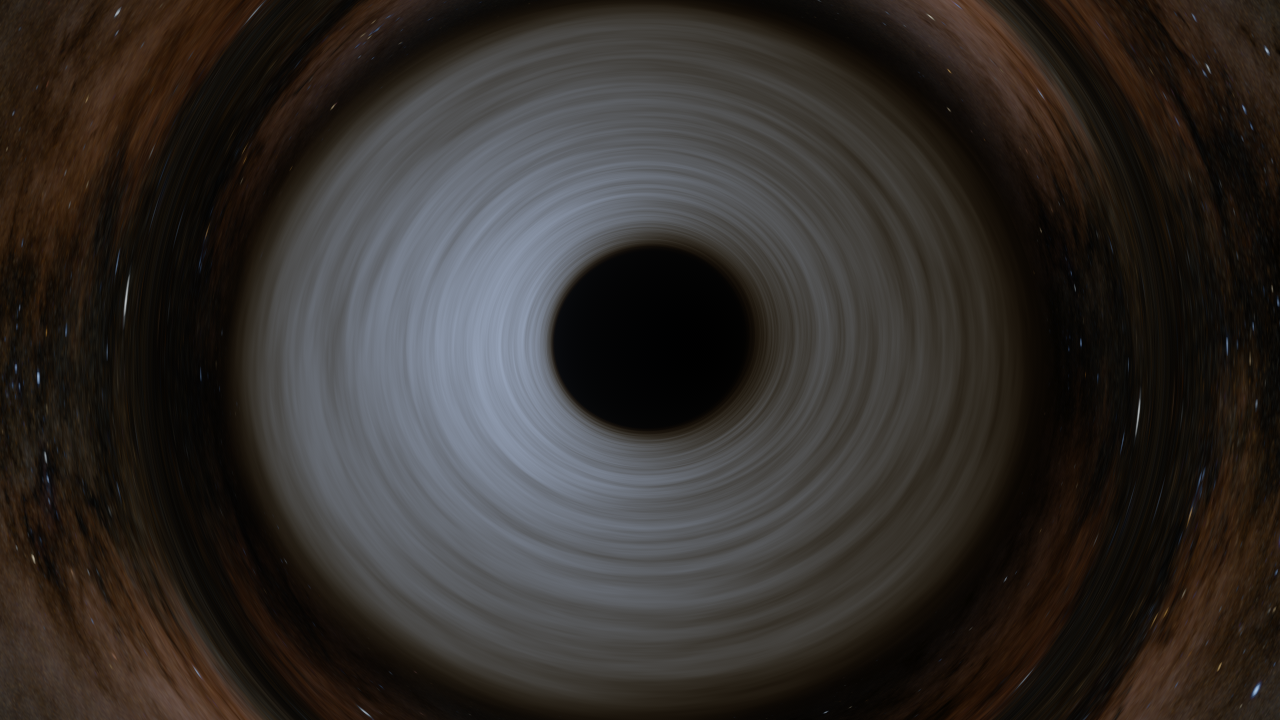
\includegraphics[width=0.82\textwidth]{figures/x_preset1_earth.png}
\vfill
{\large C.~Excelsis\par}
\vspace{0.3cm}
{\large Independent research report --- companion to the thesis\par}
\vspace{0.3cm}
{\large \today\par}
\end{titlepage}

%---------------------------------------------------------------- contents
\pagenumbering{roman}
\tableofcontents
\listoffigures
\listoftables
\cleardoublepage

%---------------------------------------------------------------- abstract
\chapter*{Abstract}
\addcontentsline{toc}{chapter}{Abstract}

This report extends the Sgr~A* simulator of the accompanying thesis from
measuring the black hole to \emph{seeing} it: every image is now rendered as
a camera would record it, from any observer's eyes, with time-dependent
sources --- and every new number is again produced by tested code. All
scenes use one spacetime, Sgr~A* with $\astar = 0.94$ and the GRAVITY mass and
distance.

(i)~\emph{Spectral rendering.} A redshifted blackbody is a blackbody at
$gT$, so one Planck--CIE lookup carries Doppler colour and beaming. The live
GPU renderer now reproduces the fp64 CPU reference pixel for pixel (median
luminance difference \XLiveDlnYMed, 95th percentile \XLiveDlnYPninetyfive\,\%;
Doppler contrast within \XLiveBeamErr\,\%). A thin disk fed at Sgr~A*'s
measured accretion rate would peak at $\XTpeakLow$--$\XTpeakHigh$\,K and shine
$\XLumFactorLow$--$\XLumFactorHigh$ times brighter than Sgr~A* actually does
--- a quantitative reason its real accretion flow cannot be a thin disk. A
camera's Doppler contrast differs from the bolometric $g^4$ law: stronger
below $\approx\XContrastCrossT$\,K, weaker above.
(ii)~\emph{A horizon-penetrating integrator.} Cartesian Kerr--Schild
Hamiltonian geodesics with an analytic gradient replace the Boyer--Lindquist
live kernel, removing its polar seam.
(iii)~\emph{Observers.} Static, orbiting, free-falling and hovering
observers see the aberrated, Doppler-shifted sky predicted by their Lorentz-
boosted tetrads; the Schwarzschild shadow edges match Synge's formula plus
special-relativistic aberration to $\XAberrationCheck$, and the live renderer
matches the fp64 reference to $\XObsGpuMaxPx$ pixel. The comparison exposed,
and fixed, a step-budget defect that had widened the prograde edge of the
high-spin shadow by $\XLegacyBudgetPx$ pixels.
(iv)~\emph{Flares.} A Gaussian hot spot on the orbit GRAVITY fitted to the
2018 near-infrared flares ($R = 7\,M$, $i \approx 160\degr$), traced with
slow light, has a period of $\XFlGraPeriod$\,min (observed $40\pm8$\,min) and
moves clockwise as observed, but its centroid travels only $\XFlGraChord\,\muas$
in 30\,minutes against the observed $\sim$120\,$\muas$ --- reproducing,
independently, the tension GRAVITY reported between flare periods and loop
sizes. Each flash returns as a photon-ring echo $\XFlGraEchoMinMin$--$\XFlGraEchoMaxMin$
minutes later.
(v)~\emph{The hot flow at 230\,GHz.} A semi-analytic radiatively
inefficient flow, normalised to the EHT's $\XRiafTarget$\,Jy and traced with
thermal-synchrotron radiative transfer, puts its light in a Doppler-boosted
crescent inside the photon ring. Its ring, $\XRiafDraw\,\muas$, and its
first visibility minimum, $\XRiafNullMin\,{\rm G}\lambda$, are smaller than
the EHT's $51.8\,\muas$ and $3.0\,{\rm G}\lambda$: the emission must sit
further out, for instance in cooler electrons. Transported to the camera
with the Walker--Penrose constant, its polarisation shows a radial pattern
for a toroidal field, which the EHT excludes. Only a vertical, poloidal field
produces the observed spiral ($\angle\beta_2 = \XPolVerArgCw\degr$ for
clockwise rotation).

(vi)~\emph{Forecasts for S2.} Fisher forecasts from the thesis' own forward
model, checked against its profile likelihood, show that the no-hair
constraint tightens much faster than the thesis' $1/\sqrt{N}$ extrapolation.
Ten more orbits of existing quality would give $\sigma(\epsq) = \XFcTenFisher$,
not $\XFcTenThesis$, because $\epsq$ acts through a secular precession. An
extended mass at GRAVITY's present bound, left out of the fit, becomes a
$\XFcBiasEpsThirtyTwo\sigma$ false no-hair signal after 32 years of
GRAVITY-quality data, invisible in the fit's $\chi^2$. Fitting it jointly
costs only a factor $\XFcInflThirtyTwo$. Frame dragging in S2's orbit needs
$\XFcLtThreeTen$ years of $10\,\muas$ astrometry for a $3\sigma$ detection.
(vii)~\emph{Falling into Sgr~A*.} A timelike geodesic in the ingoing
Kerr--Schild chart carries the camera through the event horizon, with its
conserved quantities kept to $\XIfMaxdQ$. From $\XIfRzero\,M$, the faller
reaches the horizon after $\XIfTauHorMin$ minutes of proper time, and the
inner horizon, where the model stops, $\XIfTauInsideSec$\,s later. The tidal
stretch across a 2\,m body is $\XIfStretchHor$\,m\,s$^{-2}$ at the horizon.
Ahead, the sky skimming the dark region is blueshifted up to
$\XIfEdgeZeroNineMax$-fold. The live view matches the double-precision
tracer to $\XIfGpuMaxPx$ pixel, inside the horizon as well as outside.

An appendix applies the renderer to an exotic spacetime that is \emph{not}
Sgr~A*, the traversable wormhole of \emph{Interstellar}, as a test of its
generality.

%---------------------------------------------------------------- relation
\chapter*{Relation to the thesis}
\addcontentsline{toc}{chapter}{Relation to the thesis}

This is a companion report, deliberately kept separate from the thesis. It
reuses the thesis' physics library, validation conventions and calibration
(e.g.\ one gravitational radius subtends $\UasPerM\,\muas$ and one unit of
geometric time is \XMinPerM\ minutes at the GRAVITY mass and distance), and it
cites the thesis' chapters rather than repeating them. Two thesis results are
prerequisites:

\begin{itemize}
\item the image-handedness correction (thesis Appendix ``Image handedness:
an error found and corrected''): every camera here traces the photon it
\emph{receives}; images are not mirrored;
\item the validated Carter/Mino science path, which remains the reference
against which every new renderer in this report is tested.
\end{itemize}

Display-only processing (exposure, bloom, white balance, tone curve, false
colour) is labelled wherever it appears and never enters a measurement.

%---------------------------------------------------------------- repro
\chapter*{Reproducibility}
\addcontentsline{toc}{chapter}{Reproducibility}

Every number in this report is a macro in \texttt{numbers\_ext.tex}. The
macros are written by the script \texttt{make\_numbers\_ext.py} (in
\texttt{scripts/}) from the JSON and CSV outputs of the tools listed in
Appendix~\ref{app:xrepro}. Every figure is generated by
\texttt{make\_figures\_ext.py} or rendered by a documented engine command.
\texttt{make reproduce-ext} regenerates all of them.

\cleardoublepage
\pagenumbering{arabic}


\chapter{Introduction}
\label{ch:xintro}

The thesis built a simulator of \sgra{} to \emph{measure} things: the size and
shape of the shadow and photon ring against the Event Horizon Telescope
\citep{EHT2022}, the mass and distance from the orbit of S2
\citep{Gillessen2017, Gravity2018, Gravity2020, Gravity2022}, and a
free-quadrupole test of the no-hair theorem. Its images were instruments ---
bisected boundaries, sub-ring decompositions, flux ratios --- and the renders
that accompanied them were illustrations.

This report asks a different question of the same spacetime: \emph{what
would one actually see?} Answering it honestly takes physics the thesis did
not need. A camera does not record bolometric intensity but a spectrum
filtered by its colour response. A moving observer sees a different sky from
a static one at the same point. The light reaching the camera now left its
source at different times along different paths, so a variable source ---
the near-infrared flares of \sgra{} --- appears smeared, delayed and echoed.
And the real accretion flow of \sgra{} is not the thin disk of the thesis'
renders at all, but a hot, optically thin plasma best seen at millimetre
wavelengths.

\section{What this extension adds}

Table~\ref{tab:phenomena} lists the phenomena the simulator now shows, the
gate of the extension plan that added each one and the chapter that
documents it. Every scene uses one spacetime --- \sgra{} with $\astar = 0.94$
\citep{EHT2022} and the GRAVITY mass and distance \citep{Gravity2022}. The
only exception, a traversable wormhole, appears in an appendix as a labelled
test of the code's generality, never as a model of \sgra{}.

\begin{table}
\centering
\caption{Phenomena added by the extension. ``Thesis'' marks what the thesis
already modelled; chapters in brackets are pending.}
\label{tab:phenomena}
\small
\begin{tabular}{p{7.4cm}cc}
\toprule
Phenomenon & Gate & Chapter \\
\midrule
Shadow, lensing, photon sub-rings, $g^4$ beaming, S2 orbit in full GR,
no-hair test & thesis & --- \\
True visual colour of a redshifted blackbody; Doppler hue shift & G13 & \ref{ch:xspectral} \\
High-dynamic-range display; a thin disk at \sgra's measured accretion rate & G14 & \ref{ch:xspectral} \\
Lensed real Milky Way panorama & G15 & \ref{ch:xspectral} \\
Horizon-penetrating Kerr--Schild integrator & G16 & \ref{ch:xks} \\
Moving observers: aberration, sky Doppler shift, time dilation, frame
dragging, light that visited the ergoregion & G17 & \ref{ch:xobs} \\
Orbiting hot spots (the GRAVITY flares) with slow light and photon-ring
echoes & G18 & \ref{ch:xflares} \\
Hot accretion flow at 230\,GHz; multi-band views & G19 & \ref{ch:xriaf} \\
Polarisation & G20 & \ref{ch:xriaf} \\
Forecasts: extended-mass bias, Lense--Thirring detectability & G22 & \ref{ch:xforecast} \\
A fall through the horizon of \sgra{} & G24 & \ref{ch:xinfall} \\
Traversable wormhole (exotic, not \sgra) & G21 & App.~\ref{app:xwormhole} \\
\bottomrule
\end{tabular}
\end{table}

\section{How the new physics is validated}

The extension keeps the thesis' rule that a picture is not evidence. Each
new capability follows the same pattern:

\begin{enumerate}
\item a \emph{CPU twin} in double precision, built on the thesis' physics
library, produces the reference numbers;
\item \emph{tests} pin the twin to closed forms wherever one exists --- the
Schwarzschild limit, Bardeen--Press--Teukolsky circular orbits
\citep{BardeenPressTeukolsky1972}, Synge's shadow \citep{Synge1966}, the
Carter constants \citep{Carter1968}, exact symmetries;
\item the \emph{live GPU path} (single precision, real time) is compared
with the twin pixel by pixel, and the agreement is quoted;
\item every number in this report is written by a tool and reaches the text
through a generated macro.
\end{enumerate}

The comparisons in step~3 are not formalities. The observer comparison of
Chapter~\ref{ch:xobs} exposed a defect in the live renderer that had shifted
the prograde edge of the high-spin shadow by $\XLegacyBudgetPx$ pixels.
While building the slow-light test of Chapter~\ref{ch:xflares}, a
reimplementation of the Carter integrator without the thesis' constraint
projection disagreed with the Kerr--Schild path at the $10^{-4}$ level, which
showed that the projection matters even at moderate inclinations.

\section{Conventions}

Units are geometric, $G = c = M = 1$, unless stated. At the GRAVITY mass and
distance one gravitational radius subtends $\UasPerM\,\muas$ and one unit of
coordinate time lasts \XMinPerM\ minutes. Cameras trace the photon they
\emph{receive} (thesis Appendix on image handedness); the default camera
looks at the hole with image-right along the local $+\hat\phi$ direction and
image-up toward the spin axis, so prograde material approaches on the left.
Inclinations are measured from the spin axis; $i > 90\degr$ views the hole
from below its equatorial plane, where prograde motion appears clockwise.

\section{Outline}

Chapter~\ref{ch:xspectral} treats colour and brightness: what a camera sees
of a redshifted blackbody, the corrected live colour pipeline, the display
chain, the hypothetical thin disk fed at \sgra's real accretion rate, and the
lensed Milky Way. Chapter~\ref{ch:xks} describes the Kerr--Schild integrator
that now drives every live image. Chapter~\ref{ch:xobs} adds observers in
motion. Chapter~\ref{ch:xflares} models the GRAVITY flares as orbiting hot
spots and compares them with the observations. Chapter~\ref{ch:xriaf}
replaces the hypothetical thin disk by \sgra's real, hot accretion flow at
230\,GHz and compares its total-intensity and polarised images with the
EHT's. The remaining chapters --- forecasts for future orbit monitoring and a
fall into \sgra{} --- will follow their gates.

\chapter{Spectral Rendering: What a Camera Sees}
\label{ch:xspectral}

The thesis measured beaming with the bolometric intensity, which scales as
$g^4$ and is the right quantity for flux ratios. A camera records something
else: the spectrum weighted by its colour response. This chapter derives
what that changes, documents the live renderer's colour pipeline (and the
defect found in it), and uses the result to ask what \sgra{} would look like
if it were fed by a thin disk at its measured accretion rate.

\section{A redshifted blackbody is a blackbody}
\label{sec:planckshift}

Along a light ray in vacuum $I_\nu/\nu^3$ is conserved
\citep[e.g.][]{RybickiLightman1979, MTW1973}. Light emitted at frequency
$\nu_{\rm e}$ and received at $\nu = g\nu_{\rm e}$ therefore arrives with
$I_\nu = g^3 I_{\nu/g}^{\rm (e)}$. For a blackbody emitter,
$I_\nu^{\rm (e)} = B_\nu(T) = (2h\nu^3/c^2)/(e^{h\nu/kT}-1)$, and
\begin{equation}
g^3\,B_{\nu/g}(T)
= g^3\,\frac{2h(\nu/g)^3/c^2}{e^{h\nu/(gkT)}-1}
= B_\nu(gT) .
\label{eq:planckshift}
\end{equation}
The received spectrum is exactly a blackbody at the observed temperature
$T_{\rm obs} = gT$. One lookup table of $B_\nu(T)$ through the CIE~1931
colour-matching functions \citep[fitted as in][]{WymanSloanShirley2013} then
carries everything at once: the Doppler and gravitational colour shift and the
beaming. Only the \emph{bolometric} integral of \eqref{eq:planckshift} is the
$g^4$ law, $\int B_\nu(gT)\,d\nu = \sigma (gT)^4/\pi$. A camera integrates
$B_\nu(gT)$ against its own spectral response instead, and that does not scale
as any single power of $g$.

\section{Visual versus bolometric Doppler contrast}
\label{sec:viscontrast}

The difference matters most where it is largest, between the approaching and
receding sides of the disk. Along the image major axis of the thesis'
reference view ($r_{\rm cam} = 1000\,M$, $i = 80\degr$, $\astar = 0.94$, disk
to $18\,M$; the Carter science tracer) the redshift factor of the disk ranges
from $g = \XGmin$ on the receding limb to $g = \XGmax$ on the approaching one.
\texttt{spectral\_tool} sums both the bolometric intensity and the visual
luminance $Y$ over the two halves of that axis (Fig.~\ref{fig:xcontrast}).

The bolometric ratio, $\XBoloContrast$, does not depend on the disk
temperature: every point scales by the same $T^4$. The visual ratio depends
on it strongly. For the thesis' reference temperature of 6300\,K a camera
sees the approaching side $\XVisContrastRef$ times brighter than the
receding one, \XVisBoloRatio\ times the bolometric contrast. The receding limb's light
is shifted out of the visible band onto the exponential Wien tail. For hot
disks the visible band sits on the Rayleigh--Jeans side, where
$B_\nu \propto T$, and the visual contrast drops below the bolometric one.
The two are equal at $T \approx \XContrastCrossT$\,K. The colour shifts with
them: at 6300\,K the hottest annulus seen at the extreme Doppler factors has
chromaticity $(x,y) = (\XAppChromX, \XAppChromY)$ on the approaching side, a
blue-white, and $(\XRecChromX, \XRecChromY)$ on the receding side, deep orange.

\begin{figure}
\centering
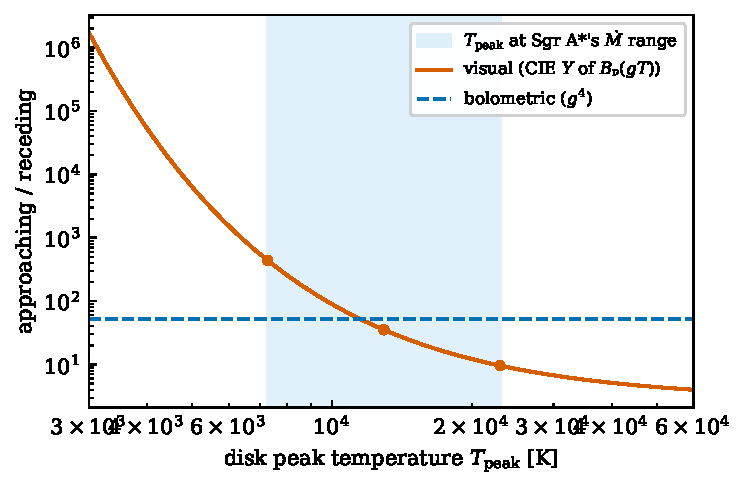
\includegraphics[width=0.75\textwidth]{figures/fig_x_contrast.pdf}
\caption{Doppler contrast between the approaching and receding halves of the
disk's major axis ($\astar = 0.94$, $i = 80\degr$, Carter tracer) as seen by a
camera (visual luminance of $B_\nu(gT)$) and bolometrically ($g^4$), versus
the disk's peak temperature. The shaded band is the peak temperature a thin
disk would have at \sgra's measured accretion rate
(\S\ref{sec:thindisk}); dots mark its three computed values.}
\label{fig:xcontrast}
\end{figure}

\section{The live colour pipeline}
\label{sec:livecolour}

The live renderer (Phases 8--15 of the thesis) coloured the disk with an
8-bit lookup table computed from the same Planck integration. Reading the
code for this extension revealed three problems:
\begin{enumerate}
\item the table stored \emph{radiance-weighted} colours,
\item it was gamma-encoded and uploaded as normalised integers,
\item the shader then multiplied by $(T_{\rm obs}/6500\,{\rm K})^4$ again.
\end{enumerate}
The temperature dependence was therefore counted twice. A 24-stop luminance
grade then mapped the result onto a narrow beige palette, which removed the
Doppler colour shift that \eqref{eq:planckshift} predicts. A separate error in
the shader's Page--Thorne flux, an extra factor $1/x^2$, made the live disk
fall off as $r^{-4}$ instead of $r^{-3}$ and run cooler than the temperature
it was given. The science path, which colours its figures with the CPU
function \texttt{planck\_to\_linear\_srgb}, was not affected.

The corrected pipeline builds a floating-point table of $B_\nu(T)$ through the
CIE curves at start-up from that same CPU function: 1024 entries,
logarithmic in $T$ from 300\,K to $10^5$\,K, normalised so that a 6500\,K
blackbody has luminance 1. The shader makes one lookup at $gT$ and nothing
else. A bolometric display mode, which shows $(gT/6500\,{\rm K})^4$ in grey,
is kept for teaching the $g^4$ law.

The validation (\texttt{compare\_live\_colour.py}) renders the thesis'
physical preset twice at identical parameters ($T_{\rm peak} = \XLiveTpeak$\,K):
once on the GPU and once with the CPU tracer and the CPU shading. Over
$\XLiveNpix$ comparable disk pixels the median luminance difference is
$|\Delta\ln Y| = \XLiveDlnYMed$ (95th percentile $\XLiveDlnYPninetyfive$\,\%),
and the median chromaticity difference is $\XLiveChromaMed$. The
approaching-to-receding luminance ratio is $\XLiveBeamCpu$ on the CPU and
$\XLiveBeamGpu$ on the GPU, a relative difference of $\XLiveBeamErr$\,\%. The
two disk footprints differ in $\XLiveMaskMismatch$\,\% of the image's pixels,
all at the one-pixel boundary between single- and double-precision tracing
(Fig.~\ref{fig:xlivecolour}).

\begin{figure}
\centering
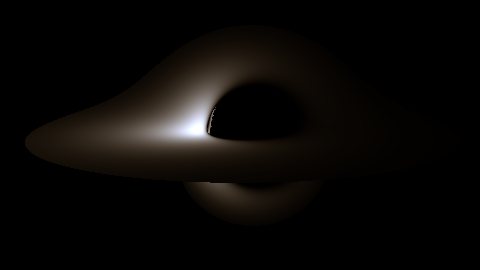
\includegraphics[width=0.49\textwidth]{figures/x_g13_cpu.png}\hfill
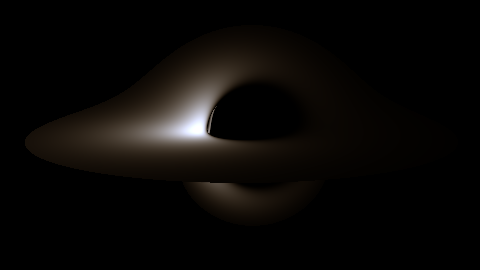
\includegraphics[width=0.49\textwidth]{figures/x_g13_gpu.png}
\caption{The physical preset ($\astar = 0.94$, $i = 80\degr$, $T_{\rm peak} =
\XLiveTpeak$\,K, linear display) rendered by the fp64 CPU reference (left) and
the live GPU path after the colour correction (right). The approaching side,
on the left, is bluer and brighter.}
\label{fig:xlivecolour}
\end{figure}

\section{The display chain}
\label{sec:display}

What a screen can show is not what the radiance image contains. Between the
two sits a display chain, applied \emph{after} the physics and switched off
completely in Science Mode, which writes the linear image with the same
transform as the CPU reference:

\begin{description}
\item[Progressive accumulation.] While the view is static, every frame adds
one jittered sample per pixel to a floating-point running mean. The jitter
follows the R2 low-discrepancy sequence \citep{Roberts2018}. Sample 0 is the
un-jittered pixel centre, so one sample reproduces the historical image
exactly.
\item[Exposure metering.] Exposure value 0 places the luminance of the
un-beamed disk at its peak temperature at display level 1, as a camera's
meter would, so disks of 7000\,K and 23\,000\,K are both well exposed.
\item[Bloom.] An energy-conserving dual-filter mip pyramid
\citep{Jimenez2014}, with a luminance-weighted first level so that single
hot pixels cannot flicker into glare.
\item[White balance and tone curve.] White-balance gains render a blackbody
of the chosen temperature neutral. A filmic curve, AgX \citep[][via the
polynomial fit of \citealt{Wrensch2023}]{Sobotka2022} or ACES
\citep{Narkowicz2016}, compresses the range while keeping hue in
overexposed regions.
\end{description}

\section{A thin disk at \sgra's real accretion rate}
\label{sec:thindisk}

The thesis' disk temperature was a display choice. Here it is computed.
Restoring $G$ and $c$ in the Page--Thorne flux \citep{PageThorne1974} gives
$F(r) = 3\mdot c^6/(8\pi G^2M^2)\,f(r)$ and $\sigma T_{\rm eff}^4 = F$. The
accretion rate of \sgra{} is bounded by the Faraday rotation of its 230\,GHz
emission to $\XMdotLow \lesssim \mdot \lesssim \XMdotHigh\,\msun\,{\rm yr}^{-1}$
\citep{Marrone2007}; see also the review by \citet{Genzel2010}. Over that
range a Novikov--Thorne disk around \sgra{} ($\astar = 0.94$) would peak at
\begin{equation}
T_{\rm peak} = \XTpeakLow\text{--}\XTpeakHigh\ {\rm K}
\qquad (\mdot = \XMdotLow\text{--}\XMdotHigh\ \msun\,{\rm yr}^{-1}),
\end{equation}
at $r = \XRpeak\,M$ ($\XTpeakMid$\,K at $\XMdotMid$). It would look
blue-white: the chromaticity at its peak moves from $(\XChromXLow,
\XChromYLow)$ to $(\XChromXHigh, \XChromYHigh)$ across the range.

Such a disk would also be far too bright. Its luminance $L = \eta\mdot c^2$,
with radiative efficiency $\eta = 1 - E_{\rm ISCO} = \XEta$ for this spin,
spans $\XLumLow$--$\XLumHigh$\,erg\,s$^{-1}$, or $\XLumEddLow$--$\XLumEddHigh$
of the Eddington luminosity ($\XLEdd$\,erg\,s$^{-1}$ at the GRAVITY mass).
\sgra{} radiates on average about $10^{-8.5}$ of its Eddington luminosity
\citep{Genzel2010}. A thin disk fed at the measured rate would therefore
outshine it by a factor $\XLumFactorLow$--$\XLumFactorHigh$. This is the
classic argument, made quantitative here, that the accretion flow of
\sgra{} is radiatively inefficient: a hot, geometrically thick, optically thin
plasma that radiates a tiny fraction of its accretion energy. That flow is
the subject of Chapter~\ref{ch:xriaf}. The thin disk survives in the renderer
as a labelled hypothetical, with its temperature computed rather than chosen
(Table~\ref{tab:xpresets}, Fig.~\ref{fig:xpresets}).

\begin{table}
\centering
\caption{The live renderer's scenes: one spacetime ($\astar = 0.94$), five
cameras and accretion rates. The thin disk is hypothetical (\S\ref{sec:thindisk});
its peak temperature follows from $\mdot$. ``Soft'' styles fade the disk's
outer rim; ``clouds'' adds an optically thin, locally thermal cloud layer
moving on the disk's own circular orbits (display only, removable).}
\label{tab:xpresets}
\small\setlength{\tabcolsep}{4pt}
% AUTO-GENERATED by scripts/make_numbers_ext.py from DiskPreset.hpp — do not edit.
\begin{tabular}{llrrrcr}
\toprule
Scene & style & $i$ [deg] & $r_{\rm cam}/M$ & $r_{\rm out}/M$ & $\dot M$ [$\msun\,{\rm yr}^{-1}$] & $T_{\rm peak}$ [K] \\
\midrule
Physical & exact & 80 & 60 & 18 & $2\times10^{-8}$ & 12\,900 \\
Earth View ($i=30\degr$) & soft & 30 & 60 & 18 & $2\times10^{-8}$ & 12\,900 \\
Close Orbit & soft, clouds & 84 & 45 & 24 & $2\times10^{-8}$ & 12\,900 \\
Low $\dot M$ & soft & 78 & 60 & 18 & $2\times10^{-9}$ & 7\,280 \\
High $\dot M$ & soft & 78 & 60 & 18 & $2\times10^{-7}$ & 23\,000 \\
\bottomrule
\end{tabular}

\end{table}

\begin{figure}
\centering
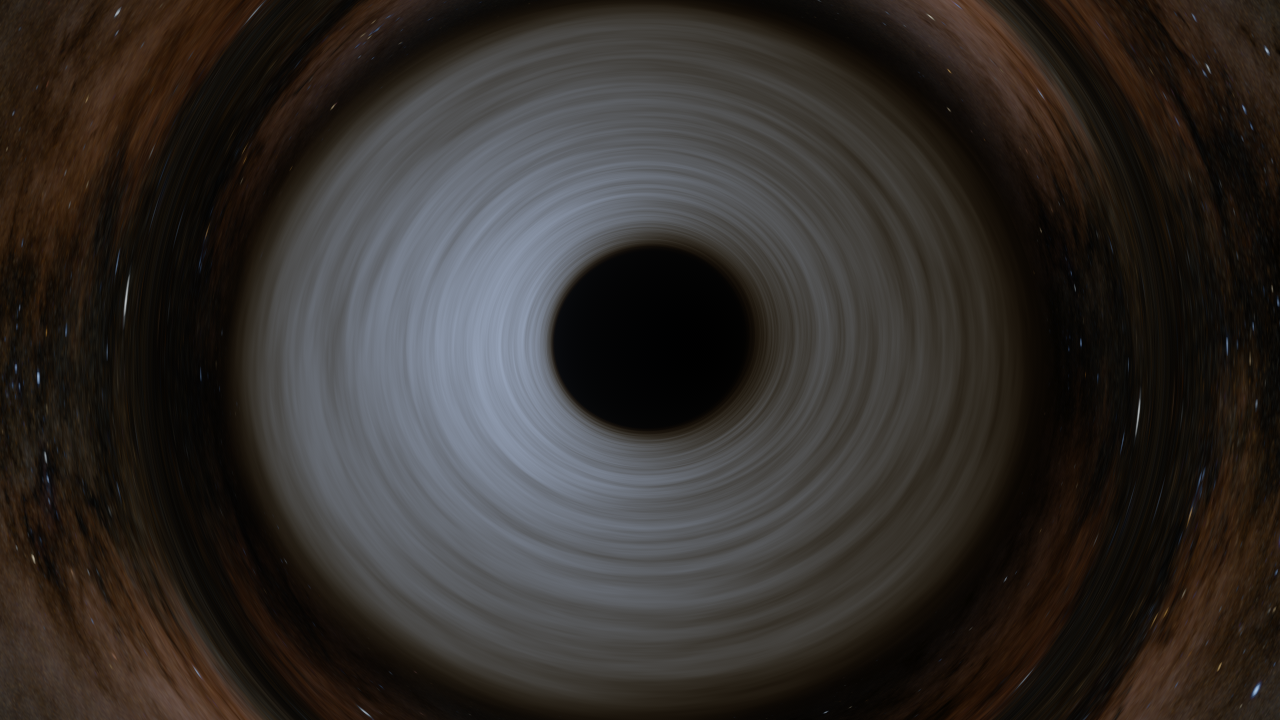
\includegraphics[width=0.49\textwidth]{figures/x_preset1_earth.png}\hfill
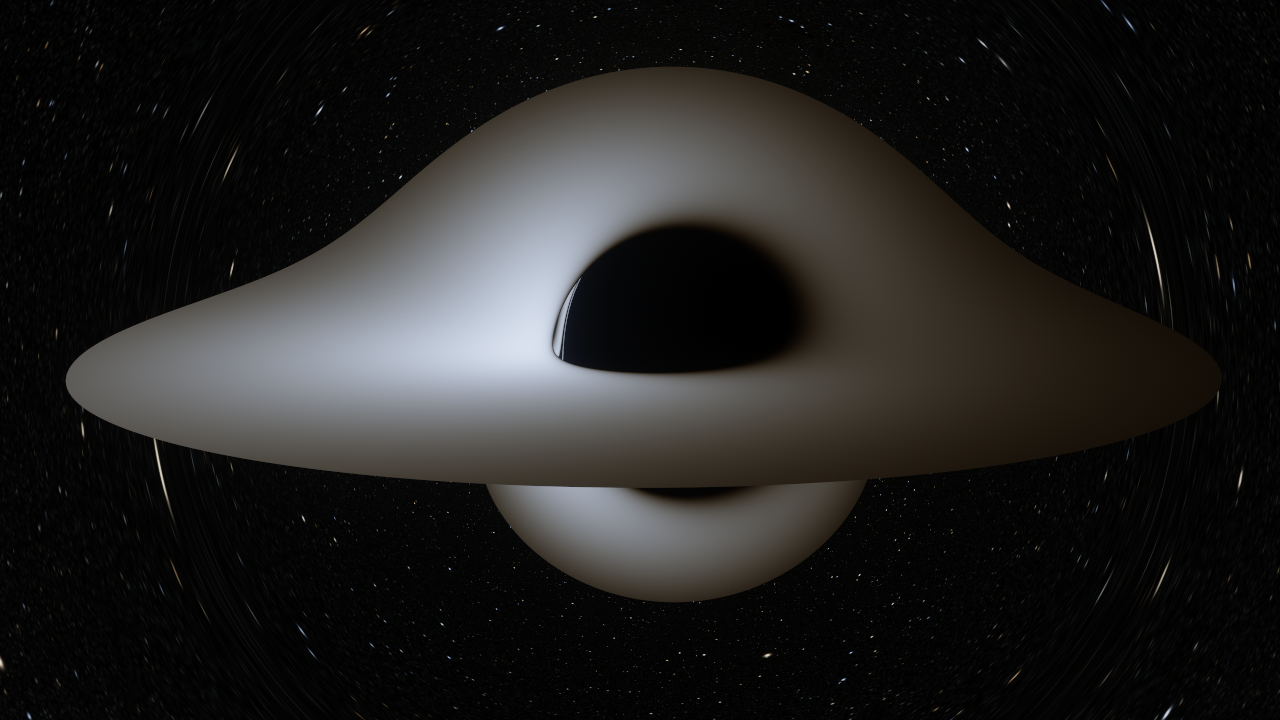
\includegraphics[width=0.49\textwidth]{figures/x_preset0_physical.png}\\[4pt]
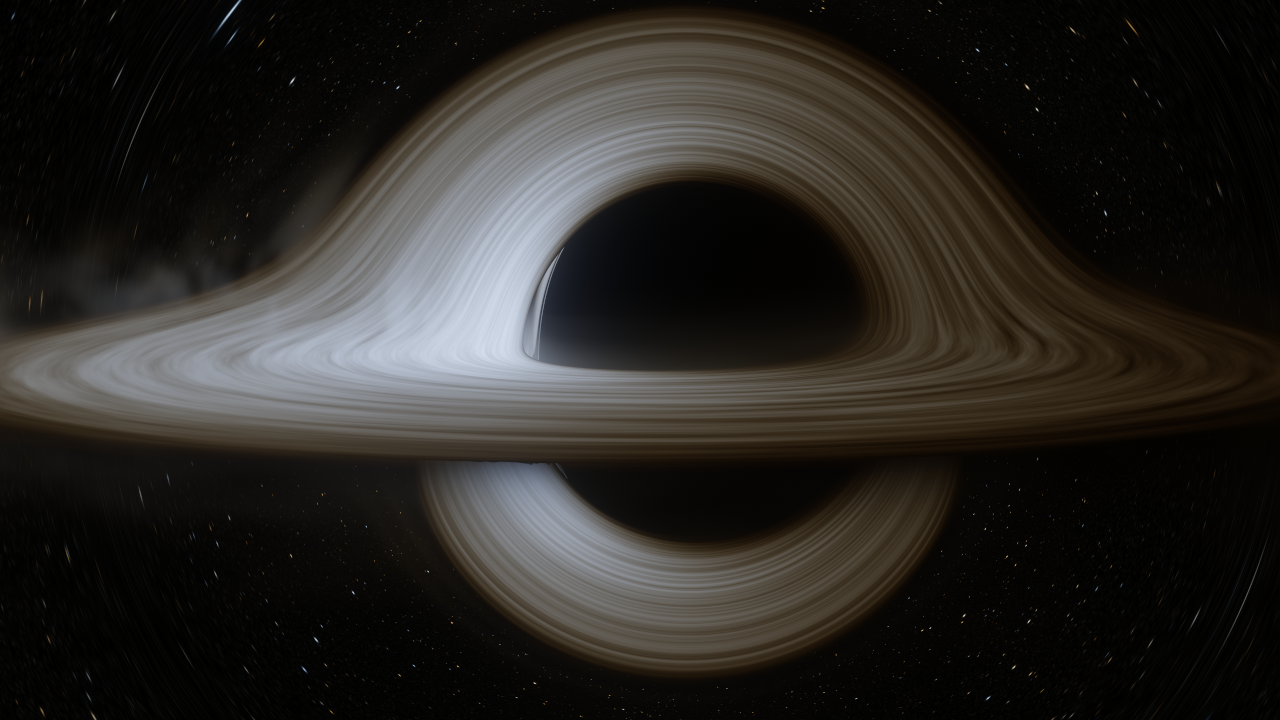
\includegraphics[width=0.49\textwidth]{figures/x_preset2_close.png}\hfill
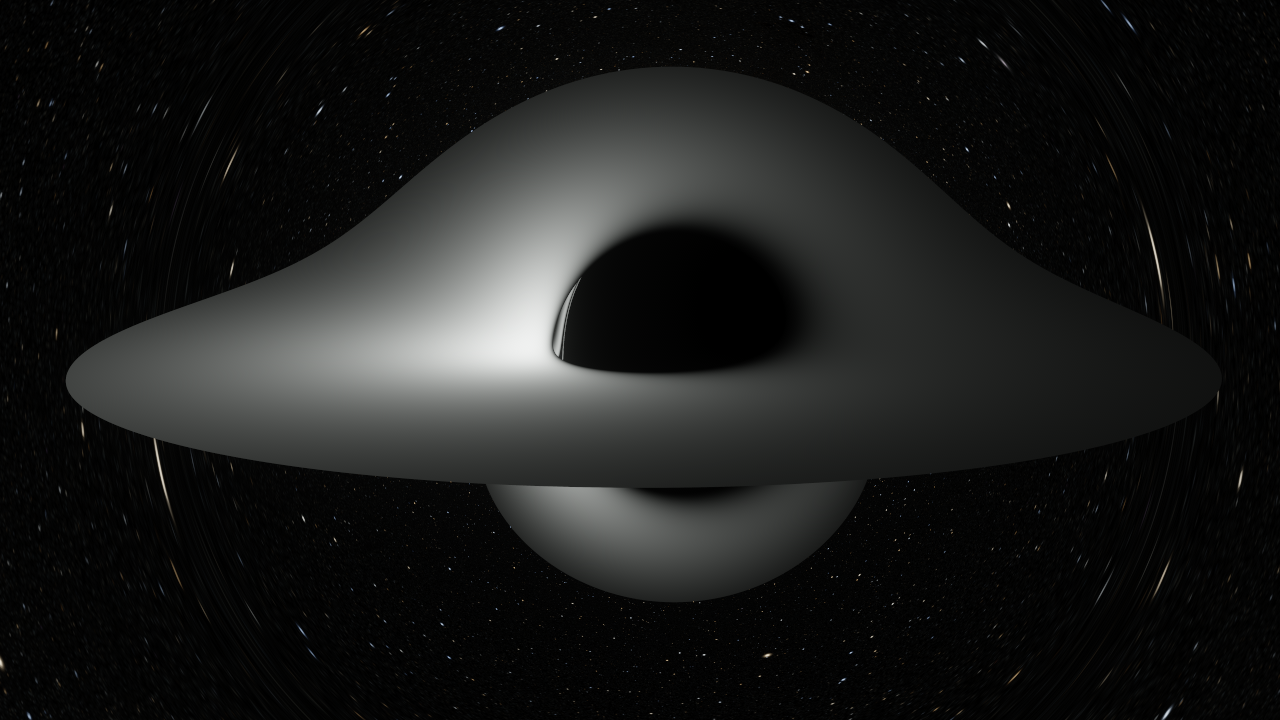
\includegraphics[width=0.49\textwidth]{figures/x_preset0_bolometric.png}
\caption{\sgra{} with a hypothetical thin disk at the computed temperature of
$\mdot = \XMdotMid\,\msun\,{\rm yr}^{-1}$. Top: the EHT viewing geometry
($i = 30\degr$, left) and the physical preset ($i = 80\degr$). Bottom left: a
close orbit with the cloud layer. Bottom right: the physical preset in the
bolometric view, which shows the $g^4$ beaming in grey. The background is the
lensed Milky Way (\S\ref{sec:sky}). Engine commands:
\texttt{scripts/render\_ext\_gallery.py}.}
\label{fig:xpresets}
\end{figure}

\section{The lensed Milky Way}
\label{sec:sky}

The thesis rendered a procedural starfield. The background is now the real
sky: the NASA SVS \emph{Deep Star Maps 2020} panorama \citep{Wright2020},
built from Gaia DR2 \citep{Gaia2018}, Hipparcos-2 and Tycho-2, in galactic
coordinates (plate carr\'ee, 8192$\times$4096). Each escaping ray reads the
map in its asymptotic direction. The texture level follows the pixel
footprint, so the dense star clouds do not alias; strongly lensed regions
alias per sample, which progressive accumulation averages away. The map is
placed with the spin axis at $i = 30\degr$ to our line of sight
\citep{EHT2022}, so a camera at that inclination sees the Galactic-Centre
star clouds behind the hole. The spin's position angle on the sky is not
constrained by current data and is set to zero, an assumption stated in the
interface.

Two caveats apply. The panorama is the sky seen \emph{from Earth}, used as a
backdrop at infinity: from the Galactic Centre, stars within a few
kiloparsecs would lie in different directions. And the map is an RGB image,
not a spectrum: when an observer's motion or gravity shifts the received
light by a factor $g$ (Chapter~\ref{ch:xobs}), each map pixel is shifted as a
6500\,K blackbody would be, $B(6500\,{\rm K}\cdot g)/B(6500\,{\rm K})$ per
channel, which gives the right sense and size of the colour and brightness
change but not a star-by-star spectrum.

\chapter{A Horizon-Penetrating Integrator}
\label{ch:xks}

The thesis integrates Carter's separated equations in Boyer--Lindquist (BL)
coordinates, in Mino time, in double precision. For metrology that is ideal:
the constants of motion are exact, and the integrator is tested to
$10^{-12}$. For a real-time renderer the same coordinates bring two problems.
The polar axis $\theta = 0, \pi$ is a coordinate singularity. Rays passing
near it needed clamps, a snap of the angular momentum and a step-squeeze
heuristic, and they still left a faint seam down the image's central column.
And the horizon is a coordinate singularity too ($\Delta \to 0$), where
backward-traced captured rays stall. This chapter describes the replacement
used by every live image of the extension: Hamiltonian geodesics in
Cartesian Kerr--Schild coordinates \citep{KerrSchild2009, Visser2007}.

\section{The Kerr--Schild form}

In Kerr--Schild form the Kerr metric is a flat metric plus a null-vector
term \citep{Kerr1963, KerrSchild2009},
\begin{equation}
g_{\mu\nu} = \eta_{\mu\nu} + f\,l_\mu l_\nu, \qquad
f = \frac{2Mr^3}{r^4 + a^2z^2},
\label{eq:ksmetric}
\end{equation}
\begin{equation}
l_\mu = \left(1,\; s\,\frac{rx + s\,ay}{r^2 + a^2},\;
s\,\frac{ry - s\,ax}{r^2 + a^2},\; s\,\frac{z}{r}\right),
\end{equation}
where the BL radius $r$ is the positive root of
$r^4 - (x^2 + y^2 + z^2 - a^2)\,r^2 - a^2z^2 = 0$ and $s = \pm1$ selects the
chart. Because $l$ is null for both $\eta$ and $g$, the inverse needs no
matrix inversion: $g^{\mu\nu} = \eta^{\mu\nu} - f\,l^\mu l^\nu$. The relation
to BL coordinates is
\begin{equation}
\begin{gathered}
x + iy = (r + i s a)\sin\theta\,e^{i\phi_{\rm KS}}, \qquad z = r\cos\theta, \\
t_{\rm KS} = t_{\rm BL} + s\,T(r), \qquad \phi_{\rm KS} = \phi_{\rm BL} + s\,\Phi(r),
\end{gathered}
\end{equation}
with $T = \int 2Mr/\Delta\,dr$ and $\Phi = \int a/\Delta\,dr$. The two charts
differ in which horizon they cover regularly. The \emph{outgoing} chart
($s = -1$) is regular across the past horizon, which is where camera rays
traced backward in time end when they fall in. The \emph{ingoing} chart
($s = +1$) is regular across the future horizon, which an in-falling observer
crosses (Chapter~\ref{ch:xinfall}).

\section{Hamiltonian equations with an analytic gradient}

With $H = \tfrac12 g^{\mu\nu}p_\mu p_\nu$ and $l\cdot p \equiv l^\mu p_\mu$, the
flat part of the inverse metric is constant, so Hamilton's equations reduce
to
\begin{equation}
\frac{dx^\mu}{d\lambda} = \eta^{\mu\nu}p_\nu - f\,l^\mu\,(l\cdot p),
\qquad
\frac{dp_i}{d\lambda} = \tfrac12\,\partial_i\!\left[f\,(l\cdot p)^2\right],
\qquad
\frac{dp_t}{d\lambda} = 0 .
\label{eq:kshamilton}
\end{equation}
The gradient follows in closed form from $\partial_i r = r(r^2x_i +
a^2z\,\delta_{iz})/(r^4 + a^2z^2)$ and the explicit $f$ and $l$. Unlike the
finite-difference gradients common in real-time renderers, this introduces
no step-size-dependent truncation error. Stationarity and axisymmetry make
$E = -p_t$ and $L_z = x\,p_y - y\,p_x$ exact constants. The Carter constant is
recovered by transforming the covector back to BL components, and $H = 0$
measures the null condition.

The double-precision twin (\texttt{physics/src/kerr\_schild.cpp}) integrates
\eqref{eq:kshamilton} with the thesis' adaptive Dormand--Prince scheme.
Cameras build their rays in BL components in the observer's frame
(Chapter~\ref{ch:xobs}), map them to Kerr--Schild components with the
Jacobian of the coordinate change, and lower them with \eqref{eq:ksmetric}.

\section{Validation}

The Catch2 suite (\texttt{test\_kerr\_schild.cpp}) checks the following:
\begin{itemize}
\item \eqref{eq:ksmetric} reproduces the BL Kerr metric, transformed, to
$10^{-12}$ at 240 points;
\item the inverse and the analytic gradient match their numerical
counterparts;
\item the Schwarzschild limit gives the critical impact parameter
$\sqrt{27}\,M$;
\item the constants of motion are conserved;
\item the camera traces the photon it receives (thesis Appendix on image
handedness).
\end{itemize}
Against the thesis' Carter tracer the image-plane comparison of the thesis
appendix gives, over $\HandKSPixels$ pixels off the spin-axis column:
\begin{itemize}
\item disk-hit radii agree to $\HandKSOffAxisDr$ and redshift factors to
$\HandKSOffAxisDg$;
\item the worst drifts along the Kerr--Schild rays are $\HandKSConsL$ in
$L_z$, $\HandKSConsQ$ in $Q$ and $\HandKSConsH$ in $H$, far inside the
thesis' $10^{-6}$ health criterion.
\end{itemize}
On the image's central column the agreement is $\HandKSAxisDr$. That column
is where BL rays pass closest to the polar coordinate singularity, so the
difference measures the reference, not the new integrator.

The time coordinate needs its own check once sources vary (Chapter~\ref{ch:xflares}).
Along a Kerr--Schild ray $dt/d\lambda = -p_t + f\,(l\cdot p)$. In the outgoing
chart the KS time of an equatorial crossing must equal the BL time from
Carter's $t$-equation plus $s\,T(r)$. The flare test suite verifies this to
$10^{-7}\,M$ for three rays of the GRAVITY flare geometry. Building that test
taught a lesson about the reference. A fresh Carter integration without the
thesis' constraint projection, which re-imposes $p_r^2 = R(r)$ and
$p_\theta^2 = \Theta(\theta)$ after every step, agreed with the Kerr--Schild
time only to $10^{-4}$ at this near-face-on inclination. It converged to the
Kerr--Schild value only as its tolerance was tightened, whereas the
Kerr--Schild result was unchanged to twelve digits at every tolerance. With
the projection restored, the two agree to $10^{-10}$.

\section{The live kernel}

The GPU kernel is a single-precision port of the twin:
\begin{itemize}
\item classical fourth-order Runge--Kutta with steps of a few per cent of
$r$, finer inside the photon region and near the disk plane;
\item bisection of each equatorial crossing on the step fraction;
\item capture at $r < r_+$;
\item for escaping rays, the asymptotic direction from the coordinate
velocity, so the background map has no parallax.
\end{itemize}
The seam heuristics of the BL kernel are gone, and the axis column renders
like any other. Three quantitative comparisons with fp64 references
underwrite it:
\begin{itemize}
\item the colour comparison of \S\ref{sec:livecolour}: $\XLiveBeamErr$\,\%
in Doppler contrast;
\item the moving-observer shadow edges of Chapter~\ref{ch:xobs}:
$\XObsGpuMaxPx$\,pixel;
\item the flare images of Chapter~\ref{ch:xflares}: centroids within
$\XFlGpuCentroidPx$\,pixel, total flux within $\XFlGpuFluxDev$\,\%.
\end{itemize}

\chapter{Whose Eyes? Observers in Motion}
\label{ch:xobs}

A black-hole image depends on who takes it. Two observers passing the same
point at different velocities see the same light arrive from different
directions (aberration), at different frequencies (Doppler shift) and with
different brightness (beaming). Their clocks also run at different rates
relative to a distant observer's. The thesis' camera was always a static
observer far away, for whom none of this matters. This chapter gives the
camera a 4-velocity.

\section{Observers and their frames}

A camera is an observer with 4-velocity $u = e_0$ and an orthonormal spatial
triad $e_i$. A pixel looking along the unit direction $n$ receives the photon
with $k \propto e_0 - n^i e_i$, which the tracer follows backward
(thesis Appendix on image handedness). The reference observer at each point
is the zero-angular-momentum observer (ZAMO) of \citet{BardeenPressTeukolsky1972},
\begin{equation}
e_{\hat t} = \frac{1}{\alpha}\left(\partial_t + \omega\,\partial_\phi\right),
\qquad
\alpha = \sqrt{-g_{tt} + g_{t\phi}^2/g_{\phi\phi}}, \quad
\omega = -\frac{g_{t\phi}}{g_{\phi\phi}},
\end{equation}
with the spatial legs along the BL coordinate directions, normalised. An
observer moving with velocity $\vec v$ relative to the ZAMO has the
Lorentz-boosted tetrad
\begin{equation}
e_0' = \gamma\,(e_{\hat t} + v^j e_{\hat j}), \qquad
e_i' = e_{\hat i} + \frac{\gamma - 1}{v^2}\,v_i\,(v^j e_{\hat j}) + \gamma\,v_i\,e_{\hat t},
\label{eq:boost}
\end{equation}
orthonormal by construction. Aberration, Doppler shift and beaming of
everything the camera sees then follow from tracing the received photons.
Nothing is added by hand. The clock rate against far-away time is
$d\tau/dt = 1/e_0'^{\,t}$.

The simulator offers five observers (\texttt{sgr\_physics/observers.hpp},
shared by the renderer and the validation tools):
\begin{description}
\item[ZAMO:] $\vec v = 0$, the frame-dragged observer.
\item[Orbiting:] circulating at the prograde Keplerian rate
$\Omega = 1/(r^{3/2} + a)$, so $v_{\hat\phi} = (\Omega - \omega)\sqrt{g_{\phi\phi}}/\alpha$.
This is a geodesic only on the equator.
\item[Free fall:] falling from rest at infinity with $E = 1$, $L_z = Q = 0$
--- the ``rain'' frame of \citet{HamiltonLisle2008} --- with
$v_{\hat r} = -\sqrt{2Mr(r^2+a^2)/A}$. For this observer $\gamma = 1/\alpha$
exactly and there is no polar motion.
\item[Hovering:] at rest relative to the distant stars ($u \propto
\partial_t$), so $v_{\hat\phi} = -\omega\sqrt{g_{\phi\phi}}/\alpha$. This
observer needs a rocket, and becomes impossible ($v \to c$) at the
ergosphere $r_E(\theta) = M + \sqrt{M^2 - a^2\cos^2\theta}$.
\item[Riding an S-star:] the star's coordinate velocity from its full-GR
orbit, the same orbit model the thesis fits to the data (S2 passes
pericentre at about 2.5 per cent of light speed, \citealp{Gravity2018}).
\end{description}

The test suite (\texttt{test\_observers.cpp}) checks these closed forms:
\begin{itemize}
\item every tetrad is orthonormal to $10^{-12}$;
\item the orbiting observer's $u^t$, $E$ and $L$ are those of the BPT72
circular orbit;
\item the free-fall observer has $u_t = -1$ and $u_\phi = 0$ at every
$(r, \theta)$;
\item the hovering observer's $u^t$ is $1/\sqrt{-g_{tt}}$;
\item hovering is valid at $1.001\,r_E$ and invalid at $0.999\,r_E$.
\end{itemize}

\section{Clocks and speeds}

Table~\ref{tab:xobs} lists each observer's speed relative to the local ZAMO
and its clock rate at three radii on the equator. The Schwarzschild entries
reproduce textbook values: at the ISCO ($r = 6M$) the circular orbit moves at
$\XIscoSpeedSchw\,c$ and its clock runs at $d\tau/dt = \XIscoClockSchw =
1/\sqrt2$, and the free-falling clock runs at $\alpha^2 = 1 - 2M/r$. For
\sgra's spin the hovering observer at $6M$ must already move at
$\XHoverSpeedSix\,c$ against the frame dragging just to stay still. The
free-falling observer reaches $\XInfallSpeedHorizon\,c$ relative to the ZAMO
at $1.001\,r_+$ ($r_+ = \XRplus\,M$).

\begin{table}
\centering
\caption{Speed $v$ relative to the local ZAMO [$c$] and clock rate
$d\tau/dt$ (observer proper time per unit far-away time) of the four
standard observers on the equator (\texttt{observer\_tool}).}
\label{tab:xobs}
\small
% AUTO-GENERATED by scripts/make_numbers_ext.py — do not edit by hand.
\begin{tabular}{rr cc cc cc cc}
\toprule
& & \multicolumn{2}{c}{ZAMO} & \multicolumn{2}{c}{orbiting} & \multicolumn{2}{c}{free fall} & \multicolumn{2}{c}{hovering} \\
$\astar$ & $r/M$ & $v$ & $d\tau/dt$ & $v$ & $d\tau/dt$ & $v$ & $d\tau/dt$ & $v$ & $d\tau/dt$ \\
\midrule
0 & 60 & 0.000 & 0.9832 & 0.131 & 0.9747 & 0.183 & 0.9667 & 0.000 & 0.9832 \\
0 & 15 & 0.000 & 0.9309 & 0.277 & 0.8944 & 0.365 & 0.8667 & 0.000 & 0.9309 \\
0 & 6 & 0.000 & 0.8165 & 0.500 & 0.7071 & 0.577 & 0.6667 & 0.000 & 0.8165 \\
0.94 & 60 & 0.000 & 0.9832 & 0.131 & 0.9748 & 0.183 & 0.9667 & 0.001 & 0.9832 \\
0.94 & 15 & 0.000 & 0.9310 & 0.265 & 0.8978 & 0.365 & 0.8667 & 0.009 & 0.9309 \\
0.94 & 6 & 0.000 & 0.8181 & 0.414 & 0.7448 & 0.575 & 0.6693 & 0.063 & 0.8165 \\
\bottomrule
\end{tabular}

\end{table}

\section{What they see}
\label{sec:xaberration}

Figure~\ref{fig:xobsrenders} shows the same place --- the camera position
of the close-orbit scene (Table~\ref{tab:xpresets}) --- through three
observers' eyes. The free-falling
observer sees the shadow and disk shrink toward the direction of motion and
brighten and blue-shift: light from ahead is aberrated forward. The orbiting
observer sees the whole scene displaced toward its direction of motion,
brighter ahead and dimmer behind.

\begin{figure}
\centering
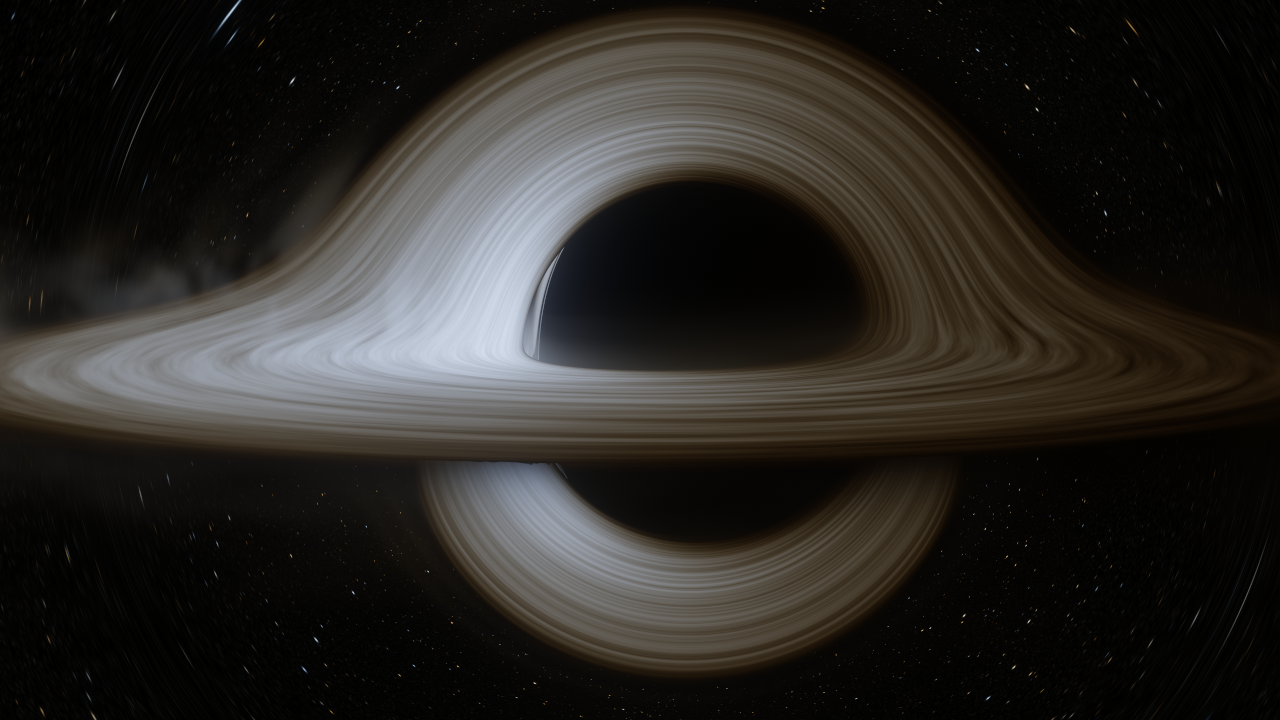
\includegraphics[width=0.32\textwidth]{figures/x_obs_zamo.png}\hfill
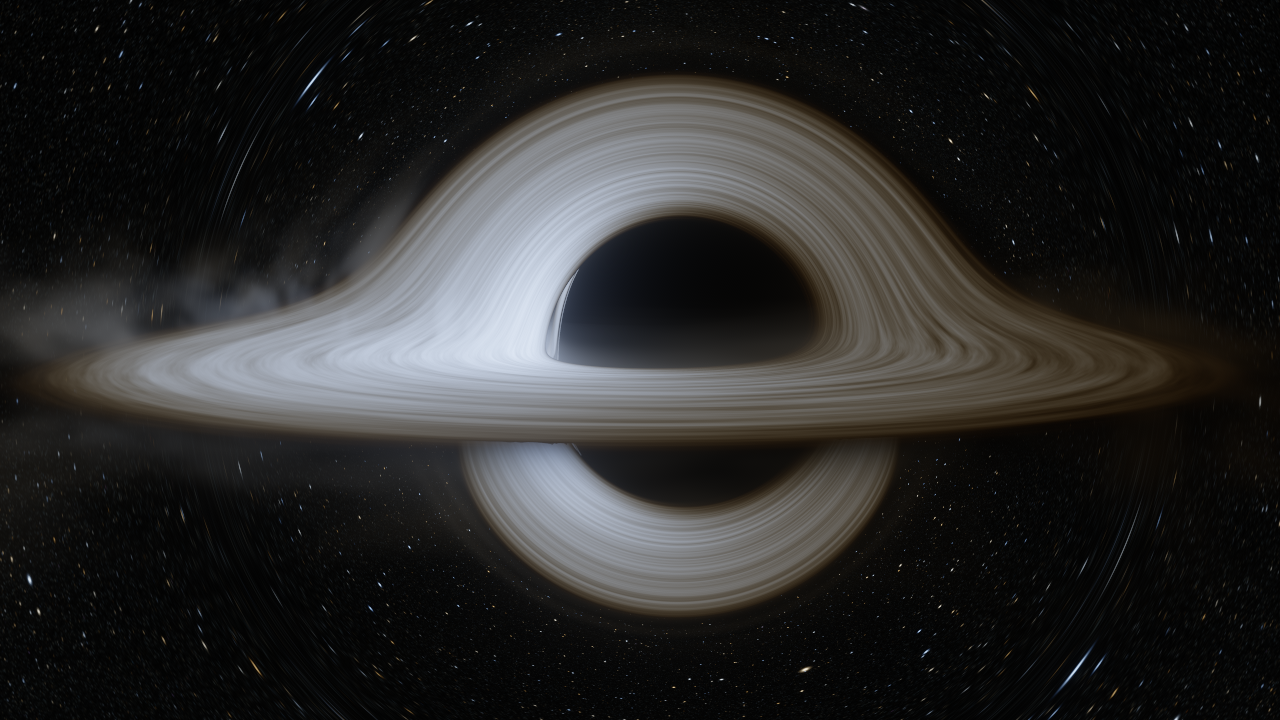
\includegraphics[width=0.32\textwidth]{figures/x_obs_infall.png}\hfill
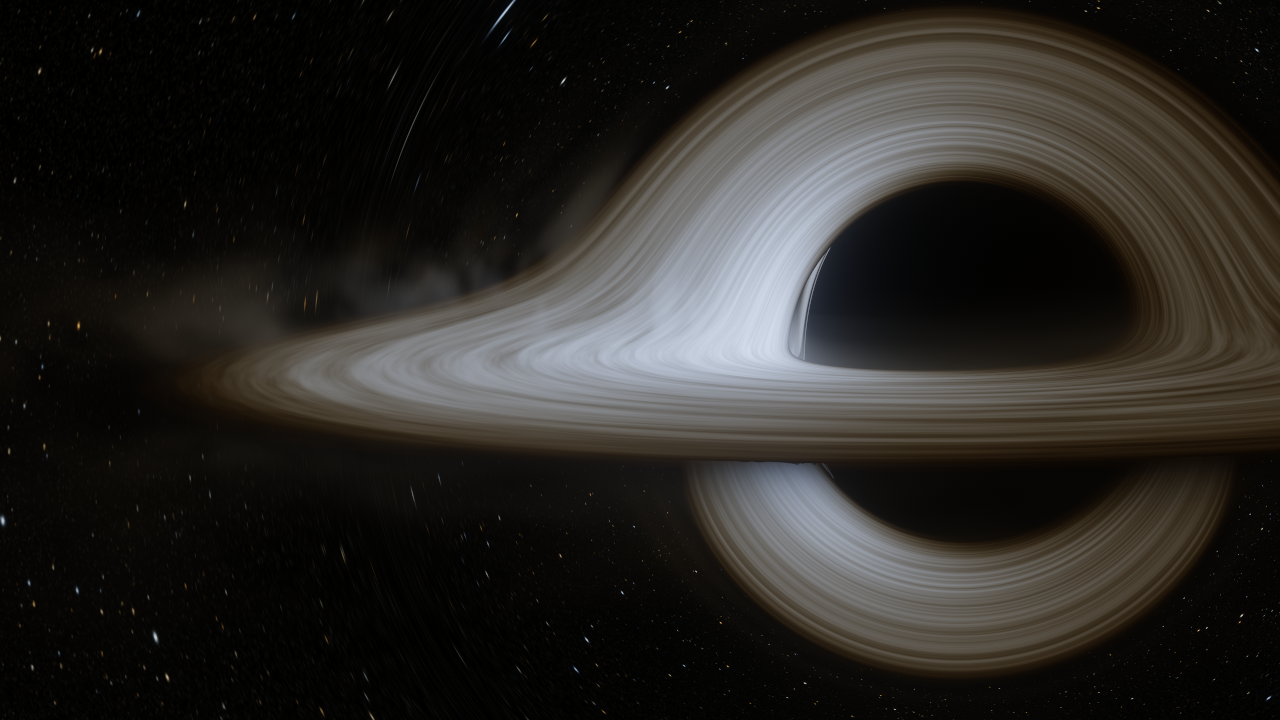
\includegraphics[width=0.32\textwidth]{figures/x_obs_orbit.png}
\caption{One place, three observers: the close-orbit scene seen by a ZAMO
(left), by an observer falling from rest at infinity (centre) and by one
orbiting at the Keplerian rate (right). Only the camera's tetrad differs.}
\label{fig:xobsrenders}
\end{figure}

The shadow makes these effects quantitative because its edge has a closed
form in the Schwarzschild case. A static observer at radius $r$ sees a
circular shadow of angular radius $\sin\psi = 3\sqrt3\,M\sqrt{1 - 2M/r}/r$
\citep{Synge1966}, which is $\XSyngeDeg\degr$ at $r = 10\,M$. A moving observer
sees every direction aberrated, $\cos\chi' = (\cos\chi + v)/(1 + v\cos\chi)$
for the angle $\chi$ to its velocity. Bisecting the shadow edges on the fp64
Kerr--Schild tracer with each observer's tetrad (\texttt{observer\_tool})
reproduces this prediction to $\XAberrationCheck$ in the tangent of the edge
angle:
\begin{itemize}
\item the free-falling observer ($v = \XInfallSpeedTen$) sees a shadow of
radius $\XInfallEdgeDeg\degr$;
\item the orbiting observer ($v = \XOrbitSpeedTen$) sees its edges at
$\XOrbitEdgeLeftDeg\degr$ on the trailing side and $\XOrbitEdgeRightDeg\degr$
on the leading side.
\end{itemize}
At $\astar = 0.94$ the ZAMO's shadow is already lopsided, with edges at
$\XKerrZamoLeftDeg\degr$ (prograde) and $\XKerrZamoRightDeg\degr$. The
orbiting observer's aberration carries the whole shadow past the centre of
view, to between $\XKerrOrbitLeftDeg\degr$ and $\XKerrOrbitRightDeg\degr$ on
the leading side (Fig.~\ref{fig:xedges}).

\begin{figure}
\centering
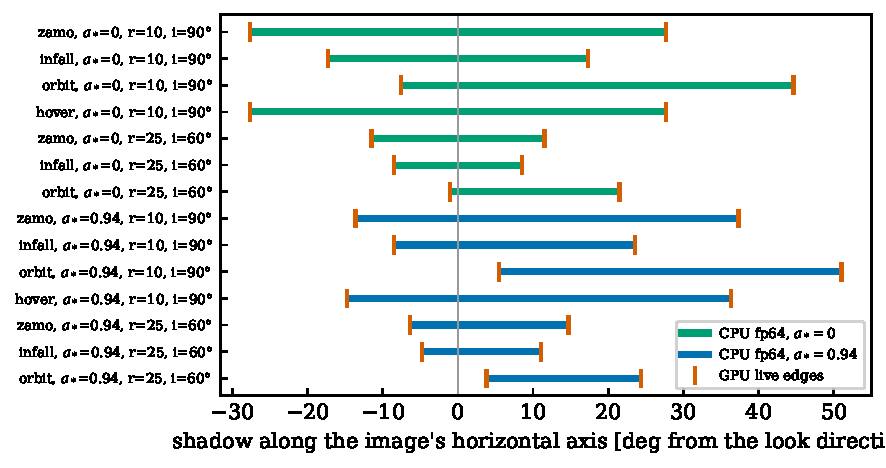
\includegraphics[width=0.85\textwidth]{figures/fig_x_observer_edges.pdf}
\caption{The shadow along the image's horizontal axis for each observer and
camera position (bars: fp64 Kerr--Schild bisection; ticks: the live GPU
renderer). At $\astar = 0$ the bars equal Synge's shadow aberrated by the
observer's velocity.}
\label{fig:xedges}
\end{figure}

\section{The sky they see}

The background shifts too. For a backward ray normalised so the camera
measures unit frequency, the conserved $p_t$ gives the ratio of received to
emitted frequency for light from infinity, $g_{\rm sky} = 1/p_t$. Deep in the
potential the sky is blueshifted by $1/\alpha$ for a ZAMO, more ahead of a
falling observer and less behind it. The renderer applies this shift to the
Milky Way map using the 6500\,K blackbody approximation of
\S\ref{sec:sky}. The effect is weak for these exterior observers, but it
dominates the view near the horizon (Chapter~\ref{ch:xinfall}).

\section{Frame dragging made visible}

Inside the ergosphere nothing can remain at rest relative to the stars, and
light is dragged too. Every captured ray crosses the ergosurface, so tinting
those rays would only colour the shadow. The overlay instead marks the light
that went \emph{inside} $r_E$ and still escaped. That set is not symmetric. At
$\astar = 0.94$ the prograde equatorial photon orbit, at $\XRphPro\,M$, lies
inside the ergosphere ($\XRergoEq\,M$ on the equator), while the retrograde
one, at $\XRphRetro\,M$, lies outside it. Only light passing on the prograde side can visit
the ergoregion and return, and it does so in a thin crescent hugging that
side of the shadow (Fig.~\ref{fig:xergo}). The crescent is a direct picture
of frame dragging.

\begin{figure}
\centering
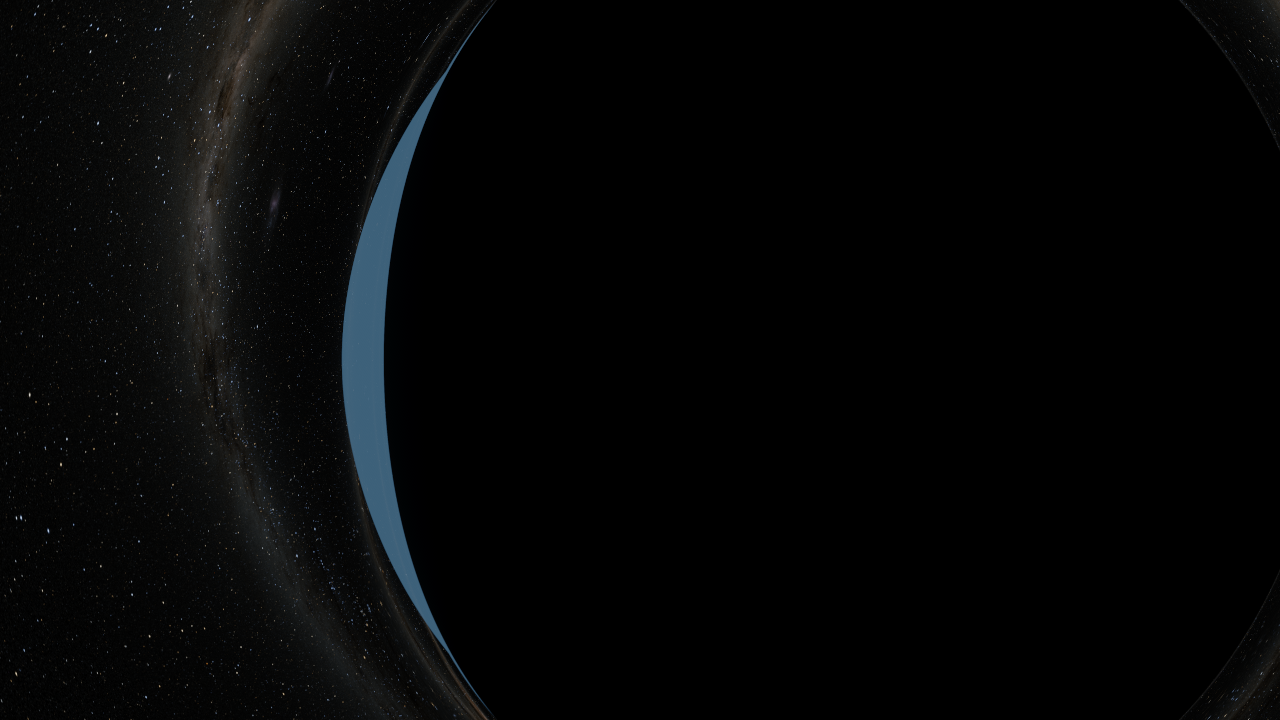
\includegraphics[width=0.7\textwidth]{figures/x_ergo_crescent.png}
\caption{Light that passed through the ergoregion and escaped (blue overlay)
around \sgra{} seen nearly edge-on ($i = 88\degr$, $r = 30\,M$, no disk;
lensed Milky Way behind). Captured light is not marked. The crescent appears
only on the prograde side, where photon orbits dip inside the ergosphere.}
\label{fig:xergo}
\end{figure}

\section{Validating the live observers}
\label{sec:xobsgpu}

The live renderer receives the boosted tetrad~\eqref{eq:boost}, computed in
double precision by the same library function the CPU tools use and
expressed in Kerr--Schild components. \texttt{compare\_observers.py} renders a
one-pixel-high strip through the image centre against a uniform sky, with no
disk, so captured rays are exact zeros. It then compares the GPU shadow edges
with the fp64 edges for $\XObsGpuCases$ observer and spin configurations. The
largest difference is $\XObsGpuMaxPx$ pixel (one pixel is $\XObsGpuPixel$ in
the tangent of the angle).

That agreement came only after the comparison found a defect. The live
kernel gave each ray at most $\XLegacyBudgetSteps$ steps and counted a ray
that exhausted them as captured. Near the high-spin prograde photon orbit
($r = \XRphPro\,M$ at $\astar = 0.94$) the orbit is only weakly unstable. A ray one
pixel from the shadow edge winds several times at about a thousand steps per
orbit, ran out of budget, and was wrongly darkened. Edge-on, this widened the
prograde side of the shadow by $\XLegacyBudgetPx$ pixels at the comparison's
resolution. The budget is now $\XBudgetSteps$ steps. Only rays at the photon ring use the
extra steps, and the old budget can be re-run on demand to reproduce the
record.

\chapter{Orbiting Hot Spots: the GRAVITY Flares}
\label{ch:xflares}

Several times a day the near-infrared emission of \sgra{} flares, rising
within minutes to many times its quiescent level \citep{Genzel2010}. In 2018
the GRAVITY interferometer resolved the motion of three bright flares
\citep{Gravity2018flares}. Their emission centroids traced clockwise loops on
the sky, with the polarisation angle rotating in step. On July~22 the
centroid moved by about 120\,$\muas$ in about 30 minutes, roughly 30 per cent
of the speed of light. GRAVITY's relativistic modelling located the emitter on
a near face-on circular orbit just outside the innermost stable orbit, with
best fits near $R \approx 7\pm0.5\,R_g$, $i \approx 160\degr\pm10\degr$ and a
period $P = 40\pm8$ minutes. The other two flares traced loops of total
amplitude $\sim$110--140\,$\muas$. A dedicated follow-up
\citep{Gravity2020flares} found all three flares consistent with a compact
hot spot at $R \approx 9\,R_g$ and $i \approx 140\degr$, and noted a tension:
the observed motion on the sky is systematically \emph{larger} than geodesic
hot-spot models predict for the observed period.

This chapter builds that model on our \sgra{} spacetime, traces it with full
slow-light ray tracing, and compares its observables with the published
ones. Every orbit and inclination below is taken from those papers; nothing
is tuned.

\section{The model}

The emitter is the one GRAVITY used \citep[][following
\citealt{BroderickLoeb2006, Hamaus2009}]{Gravity2020flares}: a Gaussian blob
of emissivity $\varepsilon \propto \exp(-d^2/2s^2)$, size $s = \XFlSigma\,M$
(their fiducial value), whose centre follows the prograde circular equatorial
geodesic of BL radius $R$, $\Omega = 1/(R^{3/2} + a)$. The blob moves rigidly
with the centre's 4-velocity $u = u^t(\partial_t + \Omega\,\partial_\phi)$, and
$d$ is the comoving distance $d^2 = (g_{\mu\nu} + u_\mu u_\nu)\,\Delta x^\mu
\Delta x^\nu$ at fixed coordinate time. The emission is optically thin, with
$j_\nu \propto \nu^{-\alpha}$. Along a backward ray normalised so the camera
measures unit frequency, conservation of $I_\nu/\nu^3$ gives
\begin{equation}
I_{\rm obs} = \int g^{2+\alpha}\,\varepsilon\,d\lambda, \qquad
g = \frac{1}{u^t\,(p_t + \Omega L_z)},
\label{eq:spotintensity}
\end{equation}
where $g$ is one number per ray for a rigidly rotating emitter. With
$\alpha = 0$ this is exactly the GRAVITY 2020 prescription, $F = \int D^2
\varepsilon\,ds$. The value $\alpha = 0.6$, one of the spectral indices
GRAVITY used to illustrate beaming \citep[their Appendix
C]{Gravity2018flares}, measures the sensitivity to that choice.

\emph{Slow light.} Each ray carries its Kerr--Schild time
(Chapter~\ref{ch:xks}). Light reaching the camera at observing time
$t_{\rm obs}$ left a point on the ray at $t_{\rm obs} + \Delta t$, when the spot
was where it was then. The simulator does not freeze the source while the
light travels.

\emph{Ray table.} The spacetime is stationary, so each pixel's ray is traced
once (fp64, adaptive Dormand--Prince) from a camera at $1000\,M$ over a field
of $\pm\XFlHalfWidth\,M$ with $\XFlPixels^2$ pixels. The tracer stores every
sample within $6s$ of the orbit, at a spacing of at most $s/5$, together with
its Kerr--Schild time and its image order: 0 for the direct image, 1 for the
first image lensed around the hole. Any observing time and emission model is
then a sum over stored samples. Along all rays $|H|/E^2 \le \XFlMaxdH$ and
the relative drift of $L_z$ is $\le \XFlMaxdL$.

\emph{Tests} (\texttt{test\_hotspot.cpp}) cover four properties:
\begin{itemize}
\item the orbit closes after exactly $2\pi(R^{3/2} + a)$;
\item the comoving distance co-rotates with the spot;
\item the Kerr--Schild light-travel time matches Carter's $t$-equation
(Chapter~\ref{ch:xks});
\item cameras at $i$ and $180\degr - i$ record identical light curves and
mirror-image centroid tracks, as the equatorial symmetry of Kerr requires.
\end{itemize}

\emph{Numerical noise.} The lensed images are thin arcs that no affordable
grid resolves. As they move across pixels they add a pixel-scale jitter that
shrinks as $1/n$. All observables below use the first twelve harmonics of the
one-orbit series, which removes $\XFlGraNoiseFlux$\,\% (rms) from the light
curve and $\XFlGraNoiseCentroid\,\muas$ from the centroid track. At half the
resolution ($\XFlResHalf^2$ pixels) the loop size changes by $\XFlResLoop$\,\%,
the flux contrast by $\XFlResContrast$\,\% and the echo delay by
$\XFlResEcho$\,\%. These are the numerical uncertainties of the values below.

\section{Comparison with GRAVITY}

Table~\ref{tab:xflares} and Figure~\ref{fig:xflarecurves} give the results
for three orbits:
\begin{itemize}
\item GRAVITY's 2018 best fit;
\item their 2020 global fit;
\item the radius whose prograde period, for our spin and the GRAVITY 2022
mass, equals the 2018 best-fit period of 40 minutes ($R = \XRPforty\,M$).
\end{itemize}

\begin{table}
\centering
\caption{Simulated observables of an orbiting hot spot around \sgra{}
($\astar = 0.94$; $s = \XFlSigma\,M$), from \texttt{flare\_tool}. Loop: the
largest separation of two centroid positions; in brackets the geometric
orbit diameter. Chord: the largest centroid displacement within 30
minutes and the corresponding speed. Contrast: maximum over minimum flux
for $\alpha = 0$ ($\alpha = 0.6$). Lensed: mean flux fraction in images of
order $n \ge 1$. Echo: delay of the $n=1$ image of a flash behind the direct
one, over eight orbital phases.}
\label{tab:xflares}
\small
\begin{tabular}{lccc}
\toprule
& GRAVITY 2018 & GRAVITY 2020 & $P = 40$\,min \\
\midrule
$R$ [$M$], $i$ [deg] & $\XFlGraR$, $\XFlGraIncl$ & $\XFlGrbR$, $\XFlGrbIncl$ & $\XFlPfoR$, $\XFlPfoIncl$ \\
period [min] & $\XFlGraPeriod$ & $\XFlGrbPeriod$ & $\XFlPfoPeriod$ \\
loop [$\muas$] & $\XFlGraLoop$ ($\XFlGraOrbit$) & $\XFlGrbLoop$ ($\XFlGrbOrbit$) & $\XFlPfoLoop$ ($\XFlPfoOrbit$) \\
30-min chord [$\muas$] ($c$) & $\XFlGraChord$ ($\XFlGraChordSpeed$) & $\XFlGrbChord$ ($\XFlGrbChordSpeed$) & $\XFlPfoChord$ ($\XFlPfoChordSpeed$) \\
contrast & $\XFlGraContrast$ ($\XFlGraContrastSix$) & $\XFlGrbContrast$ ($\XFlGrbContrastSix$) & $\XFlPfoContrast$ ($\XFlPfoContrastSix$) \\
lensed flux [\%] & $\XFlGraLensed$ & $\XFlGrbLensed$ & $\XFlPfoLensed$ \\
echo delay [min] & $\XFlGraEchoMinMin$--$\XFlGraEchoMaxMin$ & $\XFlGrbEchoMinMin$--$\XFlGrbEchoMaxMin$ & $\XFlPfoEchoMinMin$--$\XFlPfoEchoMaxMin$ \\
\bottomrule
\end{tabular}
\end{table}

\begin{figure}
\centering
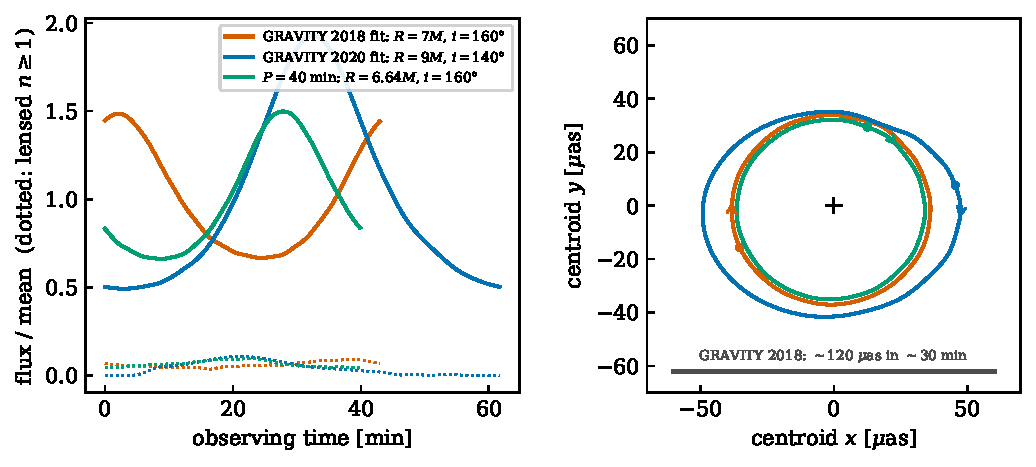
\includegraphics[width=\textwidth]{figures/fig_x_flare_curves.pdf}
\caption{Hot spots on the GRAVITY orbits around \sgra{}. Left: light curves
over one orbit, normalised to the mean (dotted: the part carried by lensed
images). Right: the flux-weighted centroid tracks on the sky (dot: start;
arrows: sense of motion; cross: the black hole). The grey bar shows the
centroid motion GRAVITY measured in the July 2018 flare, about 120\,$\muas$ in
about 30 minutes \citep{Gravity2018flares}.}
\label{fig:xflarecurves}
\end{figure}

\paragraph{Period and sense.} On GRAVITY's 2018 orbit the spot circles
\sgra{} in $\XFlGraPeriod$ minutes, inside the measured $40\pm8$. Seen from
$i > 90\degr$ its motion is \XFlGraSense{} on the sky, as observed. The 2020
orbit, at $9\,M$, takes $\XFlGrbPeriod$ minutes: within the 33--65-minute
range GRAVITY quoted as consistent with all three flares, but longer than the
July~22 best fit. The two radii bracket the problem.

\paragraph{Loop size and speed.} Lensing enlarges the apparent orbit a little
\citep[as GRAVITY's models also show;][]{Gravity2018flares}: the 2018 orbit's
centroid loop measures $\XFlGraLoop\,\muas$ against a geometric diameter of
$\XFlGraOrbit\,\muas$. Within any 30 minutes, however, the centroid moves at
most $\XFlGraChord\,\muas$ ($\XFlGraChordSpeed\,c$), about half the
$\sim$120\,$\muas$ ($\sim$0.3\,$c$) GRAVITY measured in the same interval.
Moving the spot out to $9\,M$ at $i = 140\degr$ brings the 30-minute chord to
$\XFlGrbChord\,\muas$, but at a period of $\XFlGrbPeriod$ minutes. No circular
geodesic reconciles both. This reproduces, with an independent code and our
own spacetime, the tension of \citet{Gravity2020flares}: the observed motion
is faster and larger than a hot spot on a geodesic can be for the observed
period. They discuss two partial explanations, neither modelled here:
astrometric scatter biases a measured radius upward by
$\sqrt{1 + \sigma^2/R^2}$, and the spot may move toward the observer.

\paragraph{Flux contrast.} On the 2018 orbit the light curve varies by a
factor $\XFlGraContrast$ for $\alpha = 0$ ($\XFlGraContrastSix$ for $\alpha =
0.6$). This is the combined effect of Doppler beaming, lensing and the
changing path through the blob. GRAVITY's combined orbit constraints required
a Doppler contrast below about 2.5 \citep[their Fig.~B.3]{Gravity2018flares}:
the 2018 orbit meets that with $\alpha = 0$ and only marginally with
$\alpha = 0.6$. The 2020 geometry, more inclined, varies by
$\XFlGrbContrast$. Its intrinsic heating and cooling would have to mask a
beaming signal of that size. The loop centres lie $\XFlGraOffset\,\muas$ (2018)
and $\XFlGrbOffset\,\muas$ (2020) from the black hole, well inside the
$\pm$50\,$\muas$ within which GRAVITY found them consistent with the mass
centroid.

\section{Photon-ring echoes}

Light from the spot also reaches the camera along a second path, around the
hole, as the thin lensed image in Fig.~\ref{fig:xflareimages}. That image
carries $\XFlGraLensed$ per cent of the flux on average on the 2018 orbit. Because the
second path is longer, a sudden change in the source appears twice. Flashing
the spot briefly ($\tau = 1\,M$) at eight points of its orbit and following
the direct and the first lensed image separately (Fig.~\ref{fig:xecho})
gives echo delays of $\XFlGraEchoMin$--$\XFlGraEchoMax\,M$, that is
$\XFlGraEchoMinMin$--$\XFlGraEchoMaxMin$ minutes (mean $\XFlGraEchoMeanMin$).
The echo peaks at $\XFlGraEchoPeakMin$--$\XFlGraEchoPeakMax$ per cent of the
direct flash. The delay depends on the phase because the extra path depends
on where the spot is relative to the line of sight; at the more inclined 2020
geometry it spans $\XFlGrbEchoMinMin$--$\XFlGrbEchoMaxMin$ minutes. These are
the time-domain counterpart of the thesis' photon-ring analysis: a delay set by
the mass and geometry alone, measurable in principle without resolving the
ring.

\begin{figure}
\centering
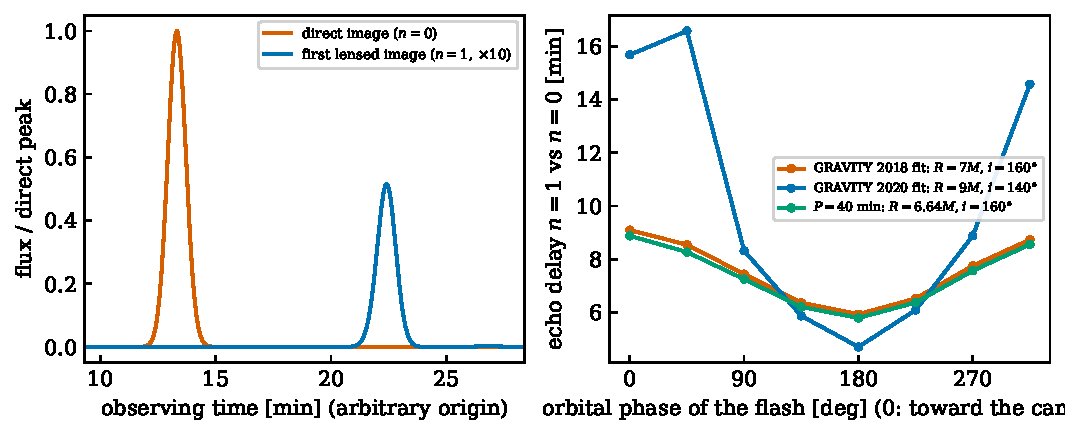
\includegraphics[width=\textwidth]{figures/fig_x_echo.pdf}
\caption{Photon-ring echoes on the GRAVITY 2018 orbit. Left: a brief flash
($\tau = 1\,M$) seen in the direct image and, delayed, in the first lensed image
(scaled up tenfold). Right: the echo delay versus the orbital phase of the
flash for the three orbits of Table~\ref{tab:xflares}.}
\label{fig:xecho}
\end{figure}

\section{The live view}

The live renderer traces the same emitter: the orbit constants and the
comoving metric are computed by the same CPU class and handed to the shader,
and each ray integrates its own Kerr--Schild time. Against the fp64 images at
four orbital phases (\texttt{compare\_flare.py}) the GPU total flux agrees to
$\XFlGpuFluxDev$\,\%, the centroid to $\XFlGpuCentroidPx$\,pixel, and the
image correlation is at least $\XFlGpuCorr$. Figure~\ref{fig:xflareimages}
shows the fp64 images. In the interactive renderer and the movie of one orbit
(\texttt{scripts/make\_flare\_movie.py}) the spot is drawn in false colour,
because 2.2\,$\mu$m synchrotron light has no visible hue.

\begin{figure}
\centering
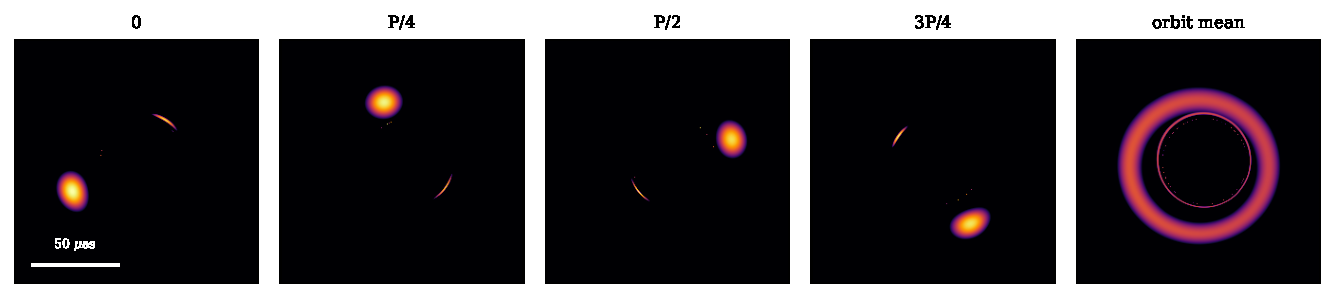
\includegraphics[width=\textwidth]{figures/fig_x_flare_images.pdf}\\[4pt]
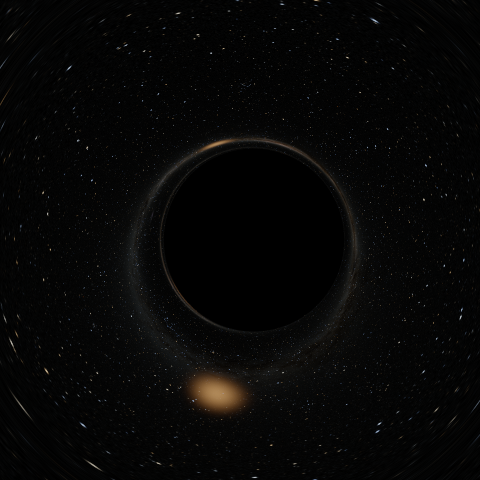
\includegraphics[width=0.24\textwidth]{figures/x_flare_0.png}\hfill
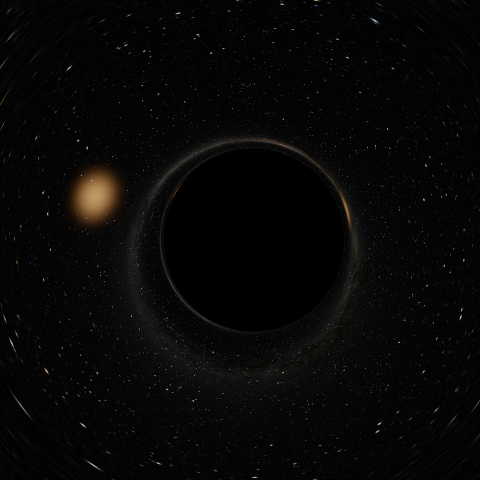
\includegraphics[width=0.24\textwidth]{figures/x_flare_1.png}\hfill
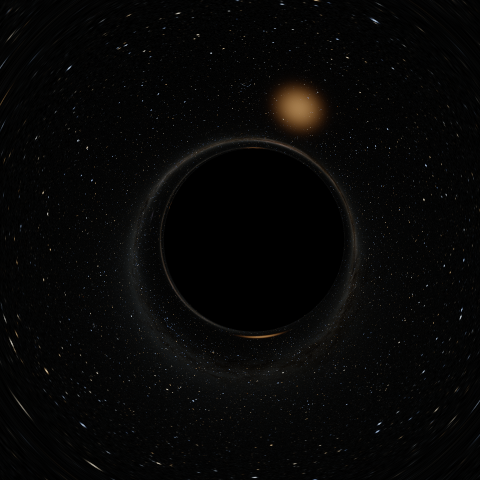
\includegraphics[width=0.24\textwidth]{figures/x_flare_2.png}\hfill
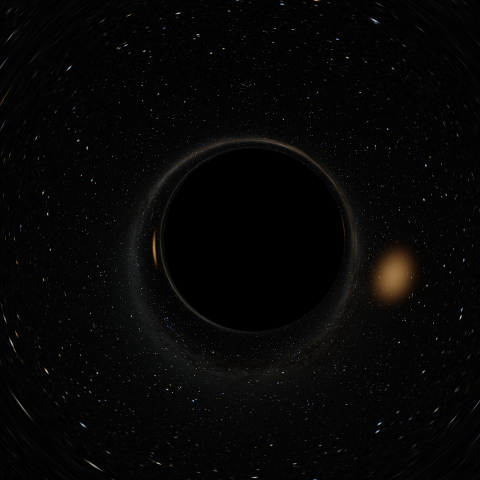
\includegraphics[width=0.24\textwidth]{figures/x_flare_3.png}
\caption{The GRAVITY 2018 hot spot around \sgra{} ($R = 7\,M$, $i = 160\degr$).
Top: fp64 images (logarithmic stretch, four decades) at quarter orbits and
averaged over one orbit; the thin arcs near the shadow edge are the lensed
images. Bottom: the live renderer at the same phases from $45\,M$, with the
lensed Milky Way behind and the spot in false colour.}
\label{fig:xflareimages}
\end{figure}

\chapter{The Hot Accretion Flow at 230\,GHz}
\label{ch:xriaf}

Chapter~\ref{ch:xspectral} showed that \sgra{} cannot be fed by a thin disk:
at the measured accretion rate one would outshine it a hundredfold. Its
accretion flow is instead hot, geometrically thick and optically thin over
most of the spectrum, a radiatively inefficient accretion flow (RIAF), and
its emission peaks at the sub-millimetre wavelengths the Event Horizon
Telescope observes. This chapter builds such a flow, traces its 230\,GHz
synchrotron emission with radiative transfer along the Kerr--Schild rays of
Chapter~\ref{ch:xks}, normalises it to the measured flux density, and
compares the result with the EHT's total-intensity \citep{EHT2022} and
polarised \citep{EHT2024pol, EHT2024polint} images of \sgra.

\section{The model}

\paragraph{Plasma.} We adopt the semi-analytic flow that Broderick and
collaborators used to interpret the first millimetre-VLBI data of \sgra{}
\citep{BroderickLoeb2006, Broderick2011}, after \citet{Yuan2003}. With
cylindrical radius $\rho$ and height $z$ (from the Boyer--Lindquist $r$ and
$\theta$), the thermal electrons have
\begin{equation}
n_e = n_0 \left(\frac{\rho}{M}\right)^{-1.1} e^{-z^2/2\rho^2}, \qquad
T_e = T_0 \left(\frac{r}{M}\right)^{-0.84},
\label{eq:riaf}
\end{equation}
with $T_0 = \XRiafTzero$\,K, the value of \citet{BroderickLoeb2006} for their
high-spin model. The field is toroidal and in partial equipartition with the
ions, $B^2/8\pi = \beta^{-1} n_e m_p c^2 r_S/12r$ with $\beta = \XRiafBeta$
\citep{Broderick2011}. The gas circulates at the Keplerian rate of its
cylindrical radius outside the innermost stable orbit and plunges inside it.
On the equator it follows the plunging geodesic with the ISCO's energy and
angular momentum. Off the plane every point takes that plunge's radial and
angular velocity at the same $r$, normalised locally. Only thermal electrons
are modelled. \citet{Broderick2011} attribute roughly 30 per cent of the
1.3\,mm flux in their models to a non-thermal population, which we omit.

\paragraph{Emission and transfer.} The thermal synchrotron emissivity is
the fit of \citet{LeungGammieNoble2011}, as implemented in grmonty
\citep{Dolence2009}:
\begin{equation}
\begin{gathered}
j_\nu = \frac{\sqrt2\,\pi e^2 n_e \nu_s}{3cK_2(1/\Theta_e)}
\left(X^{1/2} + 2^{11/12}X^{1/6}\right)^2 e^{-X^{1/3}}, \\
X = \frac{\nu}{\nu_s}, \qquad
\nu_s = \frac29\,\frac{eB}{2\pi m_e c}\,\Theta_e^2\sin\theta_B ,
\end{gathered}
\end{equation}
where $\Theta_e = kT_e/m_ec^2$ and $\theta_B$ is the angle between the photon
and the field in the fluid frame. Absorption follows from Kirchhoff's law,
$\alpha_\nu = j_\nu/B_\nu(T_e)$. Along a backward ray normalised so the camera
measures unit frequency, the fluid sees $\varepsilon = p\cdot u$, so
$\nu_{\rm f} = \varepsilon\,\nu_{\rm obs}$, and the proper length per affine
step is $\varepsilon\,\Delta\lambda$. For a thermal source the conserved
$I_\nu/\nu^3$ gives the composited solution
\begin{equation}
I_{\rm obs} = \sum_k \frac{B_{\nu_{\rm f}}(T_e)}{\varepsilon^3}
\left(1 - e^{-\Delta\tau_k}\right)e^{-\tau_k},
\qquad \Delta\tau_k = \alpha_{\nu_{\rm f}}\,\varepsilon\,\Delta\lambda\,r_g ,
\label{eq:riaftransfer}
\end{equation}
accumulated from the camera outward. Faraday rotation and conversion are
not modelled.

\paragraph{Normalisation and tests.} The density normalisation is the one
free parameter. It is fitted, by bisection on full images, so that the
230\,GHz flux density equals the EHT benchmark of $\XRiafTarget$\,Jy
\citep{EHT2022}. This gives $n_0 = \XRiafNzero$\,cm$^{-3}$. At the ISCO
the plasma then has $n_e = \XRiafNeIsco$\,cm$^{-3}$, $T_e = \XRiafTeIsco$\,K
and $B = \XRiafBIsco$\,G. Images span $\pm\XRiafHalfWidth\,M$ with
$\XRiafPixels^2$ pixels from a camera at $1000\,M$ (at $\XRiafResLow^2$ pixels
the ring diameter below changes by $\XRiafResD$\,\%), and $|H| \le
\XRiafMaxdH$ along every ray. The test suite (\texttt{test\_riaf.cpp}) checks
four properties:
\begin{itemize}
\item the flow is a unit timelike vector and the field a unit vector
orthogonal to it, inside and outside the ISCO;
\item \eqref{eq:riaftransfer} returns $B_\nu(T)$ for an optically thick
slab and $\sum j\,dl$ for a thin one;
\item $j_\nu$ is linear in $n_e$, vanishes along the field and falls off
exponentially above $\nu_s$;
\item images seen from either side of the equatorial plane are exact
mirror images.
\end{itemize}

\section{The image and the EHT ring}

Figure~\ref{fig:xriaf} shows the result at the EHT viewing geometry
($\astar = 0.94$, $i = 30\degr$). Most of the light comes from a crescent on
the approaching side. It is the direct image of the hot, Doppler-boosted
inner flow and lies \emph{inside} the photon ring, which is visible as a thin
circle at the critical curve. The inner flow's horizon silhouette, the
``inner shadow'' \citep{Chael2021}, appears as the dark spot at the centre.
The peak brightness temperature is $\XRiafTb$\,K, or $\XRiafTbBlur$\,K after
blurring with the $\XRiafBeam\,\muas$ restoring beam of the EHT's CLEAN images.

\begin{figure}
\centering
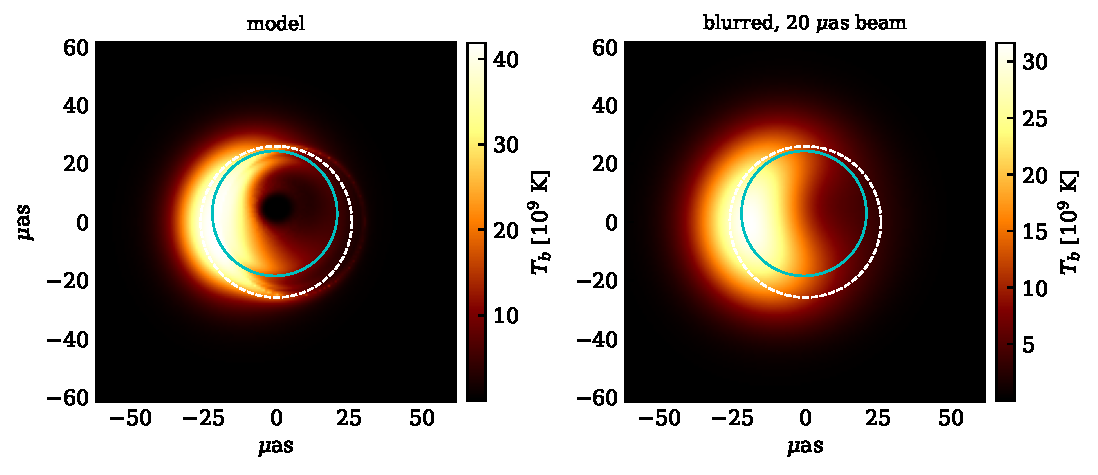
\includegraphics[width=\textwidth]{figures/fig_x_riaf_images.pdf}
\caption{\sgra{} at 230\,GHz in the RIAF model ($\astar = 0.94$, $i =
30\degr$, $n_0$ fitted to $\XRiafTarget$\,Jy), as brightness temperature.
Left: the model image. Right: blurred with the EHT's $\XRiafBeam\,\muas$
restoring beam. Dashed white: the EHT ring diameter, $51.8\,\muas$
\citep{EHT2022}; cyan: the ring measured on the model image.}
\label{fig:xriaf}
\end{figure}

The ring that the brightness peaks trace on the model image, measured as the
EHT's REx procedure does it, has a diameter of $\XRiafDraw\,\muas$ (the
centre minimises the spread of peak radii over 180 position angles). The
EHT measured $51.8\pm2.3\,\muas$. After the $\XRiafBeam\,\muas$ beam the
model's crescent is no longer resolved as a ring: its width exceeds its
diameter, $W/d = \XRiafWdBlur$. The comparison that does not depend on
resolution is the visibility amplitude: blurring multiplies the visibilities
by a Gaussian and leaves their minima where they are. The EHT found its
first and second minima at $|u| \approx 3.0$ and $6.5\,{\rm G}\lambda$,
like a thin ring of about $54\,\muas$ \citep{EHT2022}. Along the position
angles where our model shows a minimum (\XRiafNullPAs\ of 36; the lopsided
crescent fills in the others), the first lies at $\XRiafNullMin$ to
$\XRiafNullMax\,{\rm G}\lambda$. The shortest is equivalent to a thin ring of
$\XRiafThinRing\,\muas$ (Fig.~\ref{fig:xriafvis}).

\begin{figure}
\centering
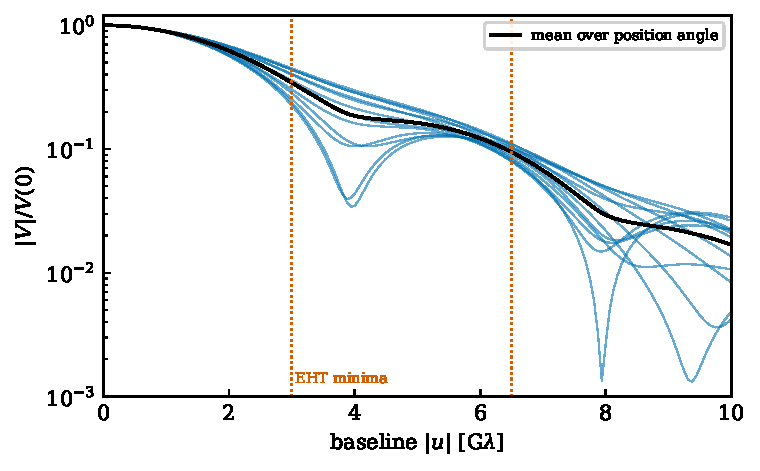
\includegraphics[width=0.78\textwidth]{figures/fig_x_riaf_vis.pdf}
\caption{Visibility amplitudes of the model image of Fig.~\ref{fig:xriaf}
along twelve baseline position angles (blue) and averaged over all (black).
Dotted: the minima of the EHT data \citep{EHT2022}. A beam does not move
these minima.}
\label{fig:xriafvis}
\end{figure}

This model is therefore too compact for \sgra. Its 230\,GHz light is
dominated by the inner flow rather than by the photon ring, and its ring is
$\XRiafRingDeficit$ per cent smaller than the one observed. This is the caveat the thesis
attached to its calibration (the measured ring tracks the critical curve
only as well as the emitting plasma sits on it), made quantitative for one
physical model. The sensitivity runs of Table~\ref{tab:xriaf} show where the
model would have to change. Halving the electron temperature moves the
emission outward and makes the image nearly symmetric: the first minimum
appears along every position angle, at $\XRiafHalfNull\,{\rm G}\lambda$
(a thin ring of $\XRiafHalfThin\,\muas$), and the brightness asymmetry drops
to $\XRiafHalfA$. A nearly face-on view ($i = 10\degr$) gives a ring of
$\XRiafTenD\,\muas$. The field strength barely matters once $n_0$ is
refitted.

\begin{table}
\centering
\caption{The RIAF at 230\,GHz: fitted density normalisation, ring diameter
on the model image, first visibility minimum (shortest over position angles;
in brackets the equivalent thin-ring diameter) and brightness asymmetry after
the $\XRiafBeam\,\muas$ beam, for the reference model and variations
(each refitted to $\XRiafTarget$\,Jy). EHT values from \citet{EHT2022}.}
\label{tab:xriaf}
\small\setlength{\tabcolsep}{4pt}
% AUTO-GENERATED by scripts/make_numbers_ext.py — do not edit by hand.
\begin{tabular}{lcccc}
\toprule
Case & $n_0$ [cm$^{-3}$] & $d$ [$\muas$] & first null [G$\lambda$] ($\muas$) & $A$ \\
\midrule
reference ($T_0$, $\beta = 10$, $i = 30\degr$) & $2.7\times10^{7}$ & 42.8 & 3.90 (40) & 0.33 \\
$T_0/2$ & $1.7\times10^{8}$ & 36.1 & 3.20 (49) & 0.08 \\
$2T_0$ & $9.2\times10^{6}$ & 47.0 & 4.45 (35) & 0.48 \\
$\beta = 3$ & $1.4\times10^{7}$ & 43.3 & 3.85 (41) & 0.35 \\
$\beta = 30$ & $5.1\times10^{7}$ & 42.5 & 3.95 (40) & 0.32 \\
$i = 10\degr$ & $3.1\times10^{7}$ & 49.2 & 3.55 (44) & 0.16 \\
$i = 60\degr$ & $2.3\times10^{7}$ & 27.2 & 4.25 (37) & 0.37 \\
\midrule
EHT 2022 (Paper I) & --- & $51.8 \pm 2.3$ & $\approx 3.0$ ($\approx 54$) & 0.04--0.3 \\
\bottomrule
\end{tabular}

\end{table}

The live renderer offers the same flow as its 230\,GHz band. With identical
parameters and pixel grid it reproduces the fp64 image to $\XRiafGpuFluxDev$\,\%
in total flux, with a correlation of $\XRiafGpuCorr$ and centroids within
$\XRiafGpuCentroidPx$\,pixel (\texttt{compare\_riaf.py}).
Figure~\ref{fig:xbands} shows one camera in the three bands the simulator now
renders.

\begin{figure}
\centering
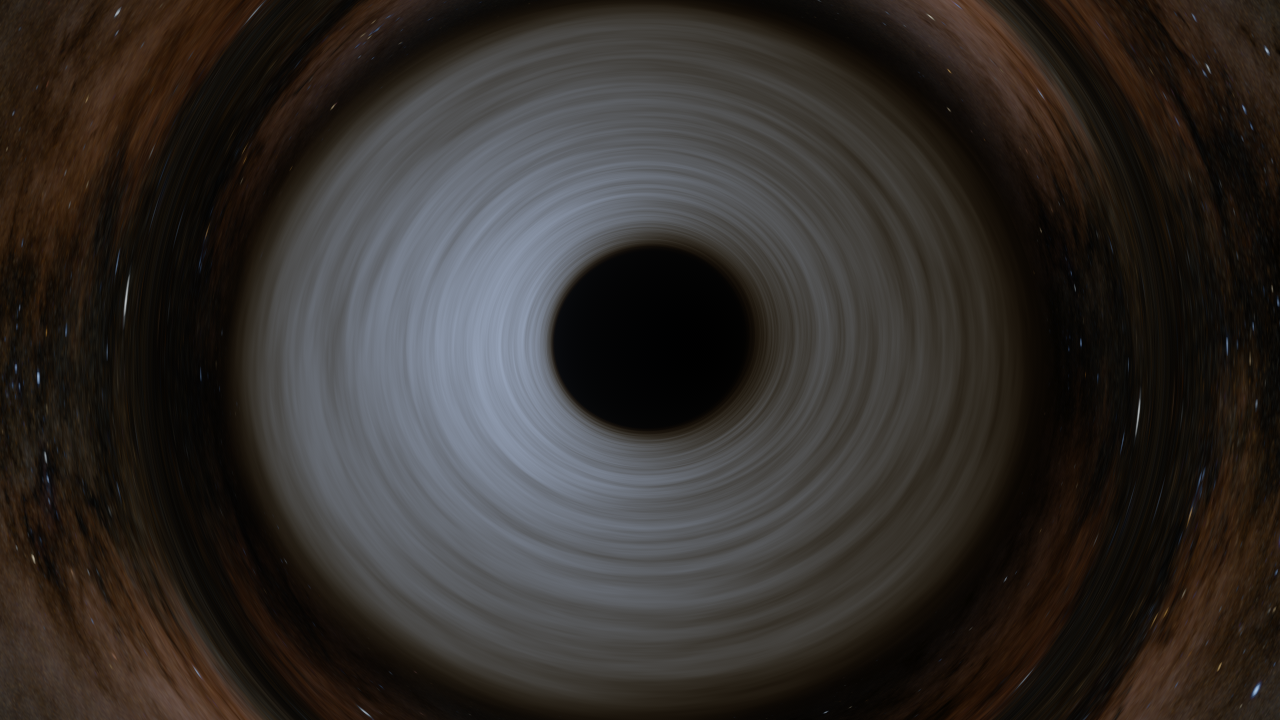
\includegraphics[width=0.32\textwidth]{figures/x_band_visible.png}\hfill
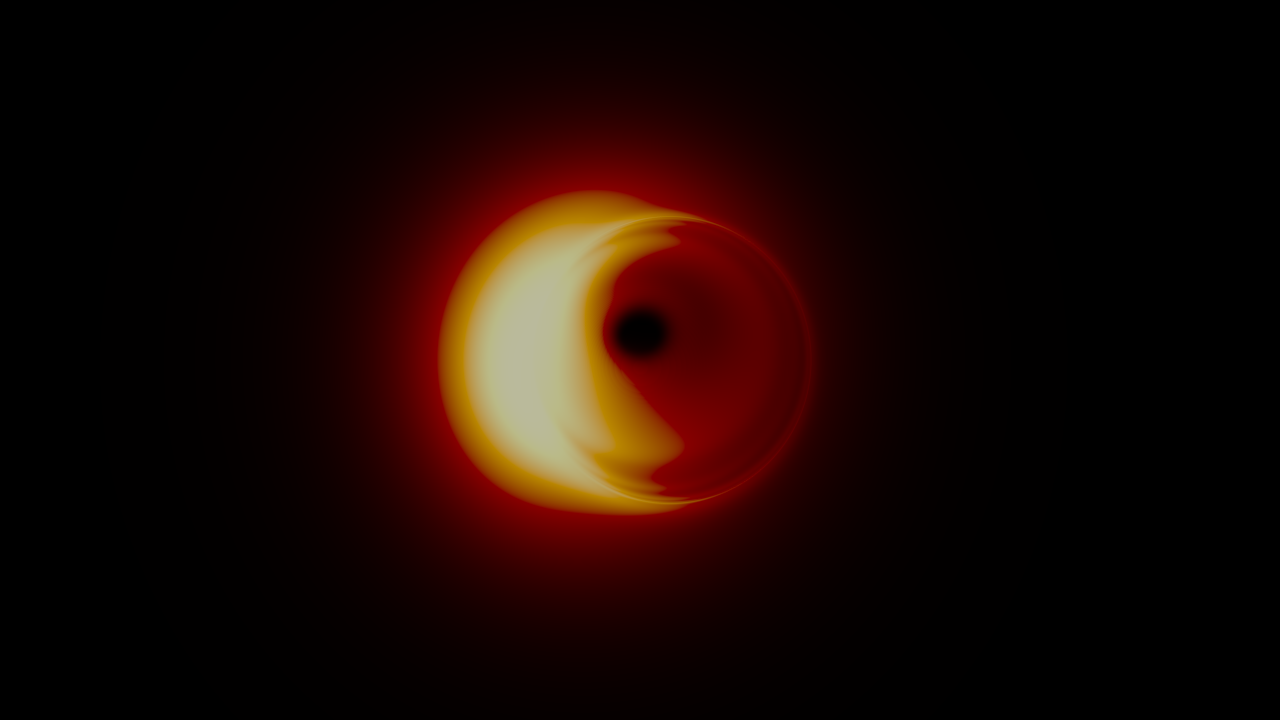
\includegraphics[width=0.32\textwidth]{figures/x_band_230.png}\hfill
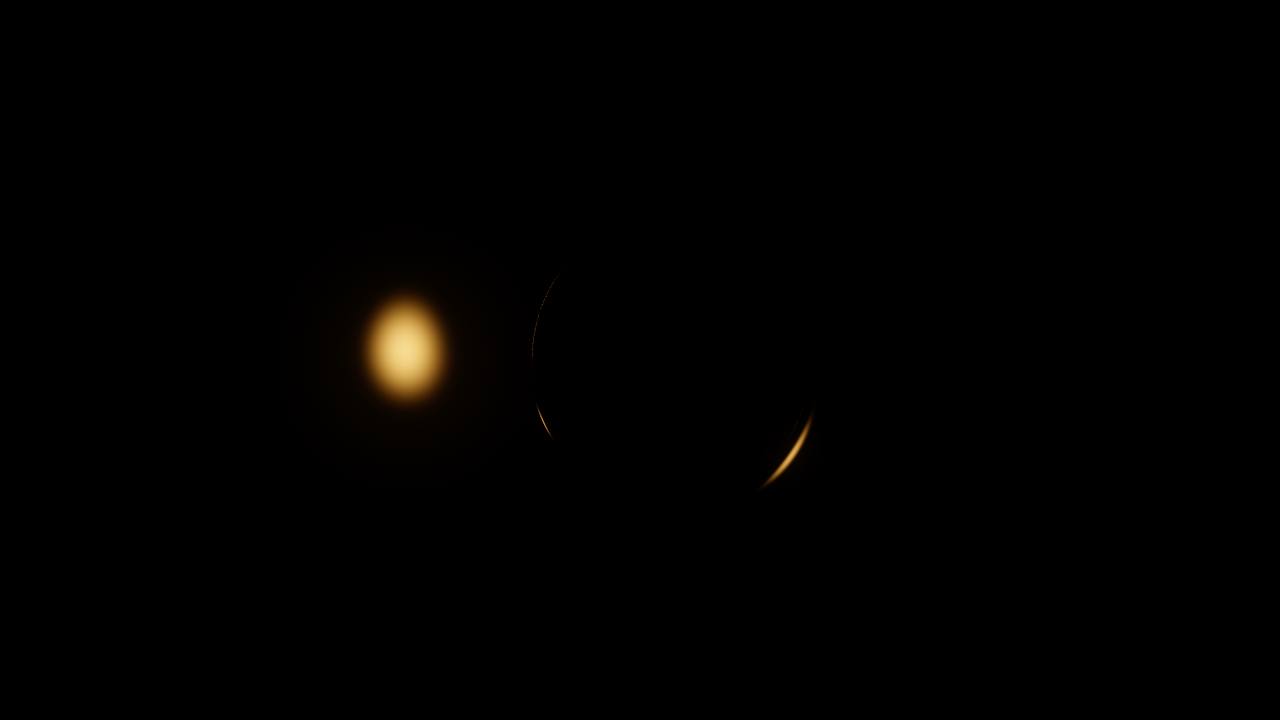
\includegraphics[width=0.32\textwidth]{figures/x_band_kband.png}
\caption{One camera ($i = 30\degr$, $60\,M$), three bands. Left: visible
light, with the hypothetical thin disk of Chapter~\ref{ch:xspectral} and the
lensed Milky Way. Centre: 230\,GHz, the hot accretion flow of this chapter
(brightness temperature, false colour). Right: 2.2\,$\mu$m, a GRAVITY hot
spot (Chapter~\ref{ch:xflares}; false colour). Only the 230\,GHz view shows
\sgra's real quiescent flow.}
\label{fig:xbands}
\end{figure}

\section{Polarisation}
\label{sec:xpol}

Synchrotron light is linearly polarised with its electric vector
perpendicular to both the photon direction and the magnetic field in the
emitting frame, $f^\mu \propto \varepsilon^{\mu\nu\rho\sigma}u_\nu k_\rho
b_\sigma$. Along a Kerr null geodesic the polarisation vector is parallel-
transported, and the \citet{WalkerPenrose1970} constant
\begin{equation}
\kappa = (A - iB)(r - ia\cos\theta), \quad
A = (k^tf^r - k^rf^t) + a\sin^2\theta\,(k^rf^\phi - k^\phi f^r),
\end{equation}
\begin{equation*}
B = \left[(r^2 + a^2)(k^\phi f^\theta - k^\theta f^\phi) - a\,(k^tf^\theta - k^\theta f^t)\right]\sin\theta
\end{equation*}
\citep{ConnorsPiranStark1980, Himwich2020} carries its orientation to the
camera without integrating the transport. At the camera the electric-vector
position angle (EVPA) is the angle $\chi$ in the image plane for which
$\kappa(\cos\chi\,e_1 + \sin\chi\,e_2)$ is a real multiple of the emission
point's $\kappa$, with $e_{1,2}$ the camera's image axes made orthogonal to
the pixel direction.

The tests (\texttt{test\_polarisation.cpp}) cover three properties:
\begin{itemize}
\item $\kappa$ is conserved to $10^{-8}$ when the polarisation vector is
parallel-transported explicitly with the Christoffel symbols along a Kerr
geodesic;
\item a face-on, non-rotating flow with a toroidal field produces a purely
radial EVPA pattern;
\item the views from either side of the equator give complex-conjugate
patterns.
\end{itemize}
Each emitting element contributes Stokes $Q + iU = p_0\,dI\,e^{2i\chi}$ with
a constant intrinsic polarisation fraction $p_0 = \XPolPzero$, an assumption.
Faraday rotation and conversion are omitted.

The EHT summarises the polarisation pattern of a ring by its azimuthal modes
$\beta_m = \sum P e^{-im\phi}/\sum I$ \citep{Palumbo2020}. The phase
$\angle\beta_2$ measures how the EVPAs twist around the ring: 0 for a radial
pattern, $\pm180\degr$ for a toroidal one. It is invariant under rotation of
the image, so the unknown orientation of \sgra's spin on the sky drops out.
Its sign follows the sense in which the flow rotates on the sky. With $p_0$
an assumption, the comparable quantities are $\angle\beta_2$ and
$|\beta_2|/|\beta_1|$, which do not depend on it.

For each field geometry we refit $n_0$ to $\XRiafTarget$\,Jy and view the
flow from $i = 30\degr$ (counter-clockwise on the sky) and $150\degr$
(clockwise, the sense of the GRAVITY flares). Table~\ref{tab:xpol} and
Fig.~\ref{fig:xpol} give the results:
\begin{itemize}
\item \emph{toroidal field} --- the electric vectors point radially,
$|\angle\beta_2| \approx \XPolTorArg\degr$. The EHT measured $\angle\beta_2$
far from zero \citep{EHT2024pol}, so a purely toroidal field is excluded;
\item \emph{radial field} --- a near-toroidal pattern,
$\angle\beta_2 = \XPolRadArgCcw\degr$ (counter-clockwise) or
$\XPolRadArgCw\degr$ (clockwise);
\item \emph{vertical (poloidal) field} --- a spiral,
$\angle\beta_2 = \XPolVerArgCcw\degr$ for counter-clockwise rotation, inside
the EHT's as-observed range of $125\degr$ to $159\degr$, and
$\XPolVerArgCw\degr$ for clockwise rotation, inside the range of $-168\degr$
to $-85\degr$ the EHT obtains after removing a constant (external) Faraday
rotation measure \citep{EHT2024pol}. Its $|\beta_2|/|\beta_1| =
\XPolVerRatio$ compares with the EHT's 1.1--2.1.
\end{itemize}
Only the poloidal field reproduces the observed spiral. That agrees with the
EHT's own interpretation, which favours flows with dynamically important
magnetic fields \citep{EHT2024polint}. Which sign of $\angle\beta_2$ applies
depends on how much of the observed rotation measure is external to the
emitting region, a question this model, which omits Faraday effects, cannot
settle.

\begin{table}
\centering
\caption{Polarisation of the RIAF at 230\,GHz for three field geometries,
seen with counter-clockwise ($i = 30\degr$) and clockwise ($i = 150\degr$)
rotation on the sky: phase of $\beta_2$ on the model and blurred images
(degrees), and on the blurred image $|\beta_2|$, $|\beta_2|/|\beta_1|$, the
resolved $\langle|m|\rangle$ and the net $|m_{\rm net}|$. $|\beta_2|$,
$\langle|m|\rangle$ and $|m_{\rm net}|$ scale with the assumed intrinsic
fraction $p_0 = \XPolPzero$. EHT 90 per cent ranges from \citet{EHT2024pol}.}
\label{tab:xpol}
\footnotesize\setlength{\tabcolsep}{3.5pt}
% AUTO-GENERATED by scripts/make_numbers_ext.py — do not edit by hand.
\begin{tabular}{lrrrrrrr}
\toprule
field & $i$ [deg] & $\angle\beta_2$ & $\angle\beta_2^{\rm blur}$ & $|\beta_2|$ & $|\beta_2|/|\beta_1|$ & $\langle|m|\rangle$ [\%] & $|m_{\rm net}|$ [\%] \\
\midrule
toroidal & 30 & +3 & +1 & 0.43 & 1.5 & 47 & 6.8 \\
toroidal & 150 & -3 & -1 & 0.43 & 1.5 & 47 & 6.8 \\
radial & 30 & -163 & -168 & 0.43 & 2.7 & 44 & 5.4 \\
radial & 150 & +163 & +168 & 0.43 & 2.7 & 44 & 5.4 \\
vertical & 30 & +133 & +135 & 0.27 & 0.8 & 42 & 12.5 \\
vertical & 150 & -133 & -135 & 0.27 & 0.8 & 42 & 12.5 \\
\midrule
EHT 2024, observed & --- & --- & 125 to 159 & 0.14--0.24 & 1.1--2.1 & 24--28 & --- \\
EHT 2024, derotated & --- & --- & $-168$ to $-85$ & & & & \\
\bottomrule
\end{tabular}

\end{table}

\begin{figure}
\centering
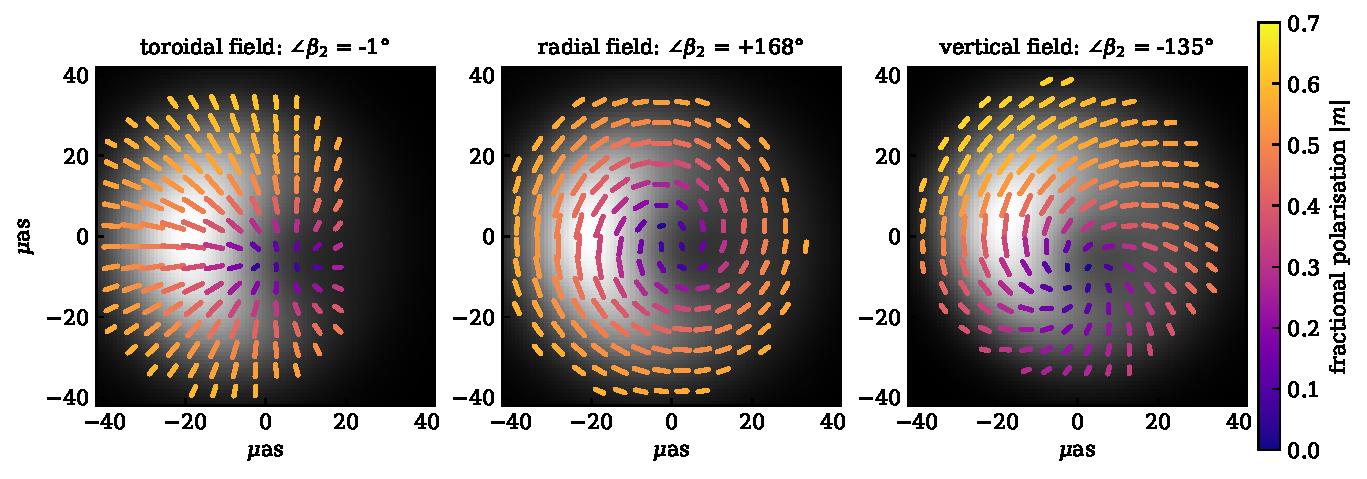
\includegraphics[width=\textwidth]{figures/fig_x_pol.pdf}
\caption{EVPA patterns of the 230\,GHz RIAF for three magnetic-field
geometries, with the flow rotating clockwise on the sky ($i = 150\degr$),
blurred with the EHT beam. Grey: total intensity. Ticks: EVPA, length
proportional to the polarised intensity, colour to the fractional
polarisation. Only the vertical (poloidal) field gives the spiral seen by the
EHT.}
\label{fig:xpol}
\end{figure}

\chapter{Forecasts for Orbit Monitoring}
\label{ch:xforecast}

The thesis measured the mass and distance of \sgra{} from the orbit of S2 and
bounded the no-hair parameter $\epsq$ with the \citet{Gillessen2017} data.
This chapter asks what continued monitoring of S2 can add, and what could
make it mislead. It uses the thesis' own forward model, the full GR orbit
with Rømer delay and relativistic redshift, on synthetic data. Four questions
are addressed:
\begin{enumerate}
\item how fast the no-hair constraint improves as orbits accumulate;
\item when S2 can reveal frame dragging;
\item how an extended mass around \sgra{} couples to the no-hair parameter;
\item how large a false no-hair signal an extended mass produces if it is
left out of the fit.
\end{enumerate}

\section{Method}

\emph{Truth and data.} The true orbit is the thesis' S2 fit, with the
reference-frame nuisances set to the centres of their priors. Noise-free
synthetic data are made with the forward model at three kinds of epochs.
\begin{itemize}
\item The real \citet{Gillessen2017} epochs and errors: $\XFcGnAst$
astrometric and $\XFcGnRv$ radial-velocity points spread over $\XFcGspan$\,yr.
\item A \emph{GRAVITY-era} continuation from 2017.0, with $\XFcGravRate$
astrometric epochs per year at $\XFcGravAst\,\muas$ per coordinate and
$\XFcGravRvRate$ radial velocities per year at $\XFcGravRv$\,km\,s$^{-1}$.
These are the precision and cadence GRAVITY reports for 2016.7--2019.7: 54
interferometric positions with rms uncertainty $\approx 65\,\muas$, and
spectra with $\approx 12$\,km\,s$^{-1}$ uncertainty taken 3--6 times a year
\citep{Gravity2020}.
\item An \emph{existing-quality} continuation that repeats the
adaptive-optics-era sampling of the \citet{Gillessen2017} data: $\XFcExRate$
positions per year at $\XFcExAst$\,mas, and $\XFcExRvRate$ radial
velocities per year at $\XFcExRv$\,km\,s$^{-1}$ (medians of those data).
\end{itemize}
Sampling is uniform in time, with no seasonal gaps, confusion or frame
systematics, so the forecasts below are idealised.

\emph{Forecasts and biases.} Forecast uncertainties come from the Fisher
matrix, $F = J^{\rm T} W J$ plus the thesis' frame priors. Here $J$ is the
central-difference Jacobian of the forward model with respect to its 13 orbit
and frame parameters, plus whichever of $\epsq$, $\astar$ and the extended
mass are free, and $W$ holds the inverse data variances.

The finite-difference steps need care. Around a pericentre passage S2 moves
fastest, along a sharply curved path, so anything
that shifts the time of passage (the mass, distance, semi-major axis or
$\epsq$) changes the predicted positions non-linearly. With the thesis' steps,
which were tuned for its imaging-era data, the Fisher matrix for the
GRAVITY-era data sets therefore depended on the steps. Here those steps are
four to eight times smaller. Halving or doubling any of them, together or one
at a time, now moves no forecast quoted in this chapter by more than
$\XFcStepCheck$ per cent.

Three further checks support the method. On the \citet{Gillessen2017} epochs,
the Fisher matrix gives $\sigma(\epsq) = \XFcSigEpsFisher$, against
$\XFcSigEpsThesis$ from the thesis' profile-likelihood fit to the real data
($\XFcSigEpsDiff$ per cent apart), and $\sigma(M)$ agrees to $\XFcSigMDiff$
per cent. For the GRAVITY-era data sets, the Fisher $\sigma(\epsq)$ agrees
with the curvature of full profile-likelihood fits within $\XFcProfAgree$
per cent (below). Biases, finally, are not linearised at all. An effect that
is present in the data but absent from the model is fitted with the thesis'
own fitter: the 13-parameter Ceres fit for $M$ and $R_0$, and the thesis'
profile likelihood in $\epsq$ (13-parameter fits at fixed $\epsq$). The
profile is not optional. Ceres differentiates numerically with a step of
$10^{-6}$ times the parameter, floored at $\sqrt{\epsilon_{\rm mach}} \approx
1.5\times10^{-8}$. At $\epsq = 0$ that step is many orders of magnitude below
any change the orbit can register, so a direct 14-parameter fit cannot move
$\epsq$ away from its starting value. The thesis' quoted best fit,
$\epsq = 0$, is that starting value. Its interval comes from the profile and
is unaffected.

\emph{The extended mass.} Stars, stellar remnants or dark matter around \sgra{}
would add a spherical mass distribution. We model it, as \citet{Gravity2020}
did, as a \citet{Plummer1911} sphere with scale radius $\XFcPlummer''$. It
enters the metric through its Newtonian potential in $g_{tt}$; its own
post-Newtonian terms are smaller by a further $O(M/r)$. Two unit tests guard
the implementation. Switched off, the model is bit-identical to the thesis
model. And a sphere ten times wider than the orbit reproduces, to within
3 per cent, the textbook retrograde precession of a homogeneous core,
$\Delta\omega = -3\pi f (a/b)^3\sqrt{1-e^2}$ per orbit. As in
\citet{Gravity2022}, its size is quoted as the fraction of $M$ enclosed
within S2's apocentre ($\XFcApo''$), which holds $\XFcEncl$ per cent of the
sphere's mass.

\section{The no-hair reach grows faster than $1/\sqrt{N}$}

The thesis extrapolated its no-hair bound by scaling the uncertainty as
$1/\sqrt{N}$ with the number of orbits. Ten further orbits of existing quality
would then shrink $\sigma(\epsq)$ by a factor $\XFcTenGainThesis$, to
$\XFcTenThesis$. The Fisher forecast for exactly that data set gives
$\sigma(\epsq) = \XFcTenFisher$, a gain of $\XFcTenGain$
(Fig.~\ref{fig:xforecast}, left).

The difference is structural. $\epsq$ acts on S2 almost only through a
\emph{secular} precession of its pericentre, and the \citet{Gillessen2017}
data contain a single pericentre passage (2002). Within one orbit, the
orientation elements absorb most of the quadrupole's effect. Each further
passage measures the accumulated advance directly, and a drift measured over a
baseline $T$ improves as $T^{-3/2}$, not $T^{-1/2}$. The jumps in the
existing-quality curve sit at the pericentre passages. The $1/\sqrt{N}$
figure in the thesis is therefore a strong underestimate of what monitoring
can achieve.

GRAVITY-era astrometry ($\XFcGravAst\,\muas$ per coordinate at $\XFcGravRate$
epochs per year, against $\XFcExAst$\,mas at $\XFcExRate$ for the
adaptive-optics data) gains faster still: $\sigma(\epsq)$ falls to
$\XFcEpsGravEight$ after 8 years, $\XFcEpsGravSixteen$ after 16 (one orbit),
$\XFcEpsGravThirtyTwo$ after 32 and $\XFcEpsGravSixtyFour$ after 64. That is
two orders of magnitude within a few decades. It is still far from the Kerr
quadrupole itself, $|\tilde q| = \astar^2 < 1$ in units of $M^3$, so S2 is
too far out to test the no-hair theorem at that level, as the thesis argued.

\begin{figure}
\centering
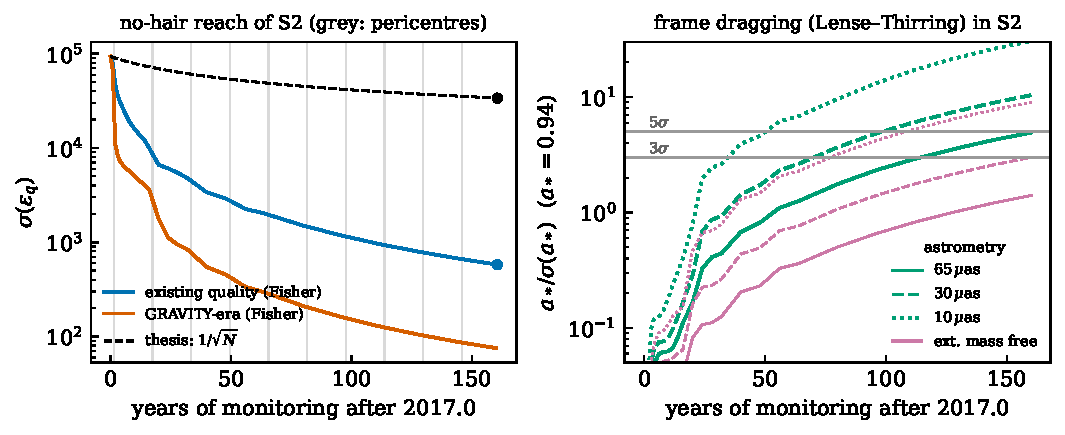
\includegraphics[width=\textwidth]{figures/fig_x_forecast.pdf}
\caption{Left: forecast uncertainty of the no-hair parameter versus
monitoring time after 2017.0, for the two continuations of the data (grey
lines: S2's pericentre passages). The dashed curve is the thesis' $1/\sqrt{N}$
extrapolation; the dots compare it with the Fisher forecast at ten more
orbits. Right: significance of the spin of \sgra{} ($\astar = 0.94$,
Lense--Thirring and Kerr quadrupole) for three astrometric precisions per
coordinate (green; purple: with an extended mass fitted at the same time).
Spin axis along the line of sight.}
\label{fig:xforecast}
\end{figure}

\section{Frame dragging}

At $\astar = 0.94$, frame dragging shifts S2's pericentre by only
$\PrecLT$~arcmin per orbit, against $\PrecSchw$~arcmin for the Schwarzschild
advance (both from the thesis' S2 fit). GRAVITY measured the Schwarzschild
advance with a 19 per cent uncertainty \citep{Gravity2020}. With $\astar$
free in the Kerr model
(Fig.~\ref{fig:xforecast}, right), the spin reaches $3\sigma$ after
$\XFcLtThreeSixtyFive$\,yr of monitoring at $65\,\muas$, and $5\sigma$ after
$\XFcLtFiveSixtyFive$\,yr. Better astrometry helps strongly: at $30\,\muas$
the times are $\XFcLtThreeThirty$ and $\XFcLtFiveThirty$\,yr, and at
$10\,\muas$ they are $\XFcLtThreeTen$ and $\XFcLtFiveTen$\,yr.

These times assume that nothing else precesses the orbit. If an extended mass
is fitted at the same time, they become $\XFcLtThreeSixtyFiveMarg$ and
$\XFcLtFiveSixtyFiveMarg$\,yr at $65\,\muas$, $\XFcLtThreeThirtyMarg$ and
$\XFcLtFiveThirtyMarg$\,yr at $30\,\muas$, and $\XFcLtThreeTenMarg$ and
$\XFcLtFiveTenMarg$\,yr at $10\,\muas$. This is the confusion that
\citet{Merritt2010} identified, and that \citet{Gravity2020} noted for their
own extended-mass limit. The direction of the spin axis matters: here it lies
along the line of sight, as throughout the thesis.

\section{The extended mass and the no-hair parameter}

An extended mass and a positive $\epsq$ both advance S2's pericentre
retrogradely, so the two parameters trade against each other. With both free,
their correlation is $\XFcCorrGs$ on the \citet{Gillessen2017} data, and
$\XFcCorrEight$, $\XFcCorrSixteen$ and $\XFcCorrThirtyTwo$ after 8, 16 and
32\,yr of GRAVITY-era monitoring. The extended mass itself is constrained to
$\sigma = \XFcSigEncGs$ per cent of $M$ within the apocentre by the
\citet{Gillessen2017} data alone, and to $\XFcSigEncEight$ per cent after
8\,yr of GRAVITY-era data. The second figure is consistent with the $\approx
0.1$ per cent that GRAVITY achieved with three years of such data
\citep{Gravity2020, Gravity2022}. Fitting the extended mass jointly costs
little: it widens $\sigma(\epsq)$ by factors of only $\XFcInflEight$,
$\XFcInflSixteen$ and $\XFcInflThirtyTwo$ at 8, 16 and 32\,yr
(Fig.~\ref{fig:xdegeneracy}, left).

\emph{Leaving it out} is a different matter (Table~\ref{tab:xbias},
Fig.~\ref{fig:xdegeneracy}, right). Take an extended mass at GRAVITY's present
$1\sigma$ bound, 0.1 per cent of $M$ within the apocentre, fitted with the
pure Kerr model. It produces a false no-hair signal of $\XFcBiasEpsEight\sigma$
after 8\,yr, $\XFcBiasEpsSixteen\sigma$ after 16\,yr and
$\XFcBiasEpsThirtyTwo\sigma$ after 32\,yr; half that mass still gives
$\XFcBiasEpsHalfThirtyTwo\sigma$ at 32\,yr. Here $\sigma$ is the uncertainty
the biased fit itself would quote, from the curvature of its profile. The
mass is biased only slightly, by $\XFcBiasMEight\sigma$,
$\XFcBiasMSixteen\sigma$ and $\XFcBiasMThirtyTwo\sigma$.

Nothing in the fit gives the problem away. Measured against the true Kerr
orbit, the extended mass alters the data by $\chi^2 = \XFcChiSignalEight$,
$\XFcChiSignalSixteen$ and $\XFcChiSignalThirtyTwo$, far more than their
errors, but the orbit elements absorb nearly all of it. The $\chi^2$ the Kerr fit leaves over is only $\XFcChiLeftEight$,
$\XFcChiLeftSixteen$ and $\XFcChiLeftThirtyTwo$. Noise alone scatters the
$\chi^2$ of these $N = \XFcNrowsEight$, $\XFcNrowsSixteen$ and
$\XFcNrowsThirtyTwo$ data values by $\sqrt{2N} = \XFcChiScatterEight$,
$\XFcChiScatterSixteen$ and $\XFcChiScatterThirtyTwo$, so the leftover is
lost in it.

That absorption also defeats linearised estimates. It moves the orbit a long
way along its best-measured direction, where the model is no longer linear.
The linear response about the true orbit recovers only
$\XFcBiasLinRatioThirtyTwo$ of the fitted 32-yr $\epsq$ bias, and for some
data sets it gets the mass bias wrong in sign. Every bias quoted here
therefore comes from a full refit.

So any future no-hair test with S2 must fit an extended mass jointly. Doing so
is cheap. Not doing so turns the extended mass, which can be no larger than
the present bound, into the leading systematic error. The thesis named this
risk in its discussion; these numbers quantify it.

\begin{table}
\centering
\caption{An extended mass (Plummer, scale $\XFcPlummer''$) present in the
data but left out of the fit: biases of the 13-parameter Kerr fit in $M$ and
$R_0$ and the $\chi^2$ it leaves, and the false no-hair signal in the thesis'
$\epsq$ profile. Noise-free data on the \citet{Gillessen2017} epochs, plus
the stated years of GRAVITY-era monitoring. For $M$ and $R_0$, $\sigma$ is the
forecast uncertainty of the same data set; for $\epsq$ it is the uncertainty
the biased fit itself would quote, from the curvature of its profile.}
\label{tab:xbias}
\small\setlength{\tabcolsep}{4pt}
% AUTO-GENERATED by scripts/make_numbers_ext.py — do not edit by hand.
\begin{tabular}{rlrrrrr}
\toprule
$M_{\rm ext}$ [\% of $M$] & data & $\Delta M/\sigma$ & $\Delta R_0/\sigma$ & $\Delta\epsilon_q$ & $\Delta\epsilon_q/\sigma$ & $\chi^2_{\rm left}$ \\
\midrule
0.05 & Gillessen 2017 & +0.02 & +0.02 & $2\,550$ & +0.03 & 0.0034 \\
0.05 & +\,8\,yr & +0.16 & +0.18 & $1\,450$ & +0.24 & 0.41 \\
0.05 & +\,16\,yr & +0.20 & +0.22 & $2\,550$ & +0.68 & 1.3 \\
0.05 & +\,32\,yr & +0.14 & +0.25 & $2\,090$ & +2.48 & 18 \\
0.10 & Gillessen 2017 & +0.05 & +0.03 & $6\,830$ & +0.07 & 0.014 \\
0.10 & +\,8\,yr & +0.32 & +0.37 & $2\,880$ & +0.47 & 1.6 \\
0.10 & +\,16\,yr & +0.42 & +0.45 & $5\,120$ & +1.36 & 5.3 \\
0.10 & +\,32\,yr & +0.35 & +0.56 & $4\,180$ & +4.98 & 73 \\
0.20 & Gillessen 2017 & +0.09 & +0.06 & $1.5\times10^{4}$ & +0.17 & 0.055 \\
0.20 & +\,8\,yr & +0.64 & +0.75 & $5\,780$ & +0.94 & 6.4 \\
0.20 & +\,16\,yr & +0.89 & +0.92 & $1.0\times10^{4}$ & +2.78 & 22 \\
0.20 & +\,32\,yr & +0.71 & +1.13 & $8\,360$ & +9.99 & 300 \\
\bottomrule
\end{tabular}

\end{table}

\begin{figure}
\centering
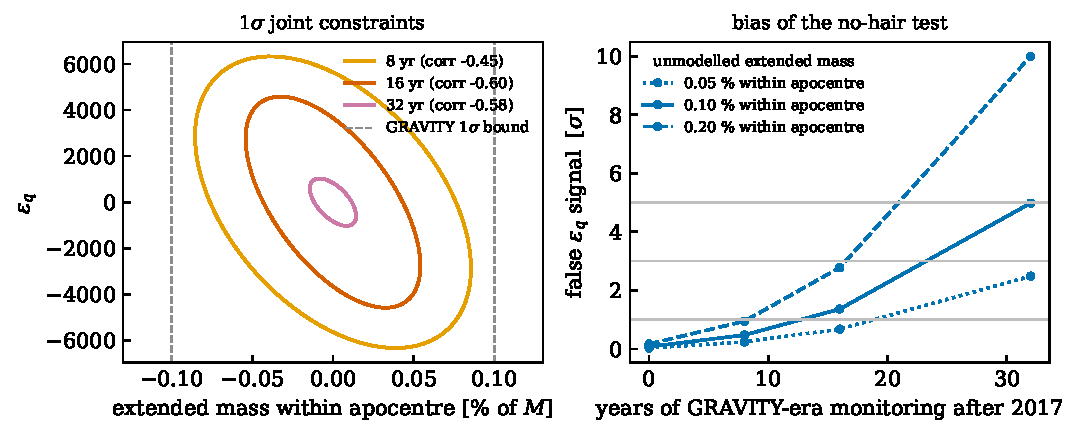
\includegraphics[width=\textwidth]{figures/fig_x_degeneracy.pdf}
\caption{Left: joint $1\sigma$ constraints on the extended mass enclosed
within S2's apocentre and the no-hair parameter, after 8, 16 and 32\,yr of
GRAVITY-era monitoring (grey: GRAVITY's present $1\sigma$ bound). Right: the
false no-hair signal, in units of the forecast $\sigma(\epsq)$, when the
extended mass is left out of the fit.}
\label{fig:xdegeneracy}
\end{figure}

\chapter{Falling into Sagittarius A*}
\label{ch:xinfall}

The last capability of the simulator is the one most often asked of a black
hole: what would someone falling in see and feel? None of it is a matter of
taste. The light, the clocks and the tides follow from the metric, and this
chapter computes each of them for \sgra{} ($\astar = 0.94$) along one
physical worldline. The fall is rendered live with every effect on.

\section{The trip}

\emph{Worldline.} A free fall is a timelike geodesic of the same Hamiltonian
the ray tracer uses, $H = \frac12 g^{\mu\nu} p_\mu p_\nu$, with $H = -\frac12$
in place of 0, so the affine parameter is the proper time $\tau$ of the
faller. It is integrated in double precision (Dormand--Prince, tolerance
$10^{-12}$) in the \emph{ingoing} Kerr--Schild chart (Chapter~\ref{ch:xks}),
which is regular across the future horizon where Boyer--Lindquist
coordinates fail. The default start is \emph{rain}: an observer dropped from
rest at infinity ($E = 1$, $L_z = 0$, $Q = 0$), whose polar angle stays
constant, the ``river'' frame of \citet{HamiltonLisle2008}. The trip begins at
$r_0 = \XIfRzero\,M$ at a polar angle of $\XIfTheta\degr$. A release
from rest relative to the local ZAMO is the alternative start.

\emph{Where it stops.} The trip ends just above the inner (Cauchy) horizon,
at $r = \XIfRstop\,M$ ($r_- = \XIfRminus\,M$). Perturbations falling in pile
up at the inner horizon and drive the mass inflation of
\citet{PoissonIsrael1990}, so the classical Kerr interior beyond it is not a
reliable description of a real black hole. The simulator says so on screen
rather than render it.

\emph{Checks.} In Schwarzschild the worldline reproduces the closed forms for
both starts: the cycloid of a fall from rest, and
$\tau = \frac23 (r_0^{3/2} - r^{3/2})/\sqrt{2M}$ for rain. The proper time to
$r = 2M$ matches them to $\XIfSchwErr$, and unit tests check radii inside the
horizon as well. For $\astar = 0.94$, across the $\XIfNsamples$ steps of the
default trip through $r_+$, $L_z$ and $Q$ are conserved to $\XIfMaxdL$ and
$\XIfMaxdQ$, and the norm of the 4-velocity to $\XIfMaxNorm$; $E = -p_t$ is
constant by construction. $Q$ is reconstructed through Boyer--Lindquist
components, so it is checked away from the two horizons, and it uses Carter's
constant for timelike geodesics. The tracer's existing routine assumed light;
this chapter generalised it.

\emph{Camera.} The faller's frame takes $e_0 = u$ and builds its three spatial
legs by Gram--Schmidt, with the full metric, from the Kerr--Schild coordinate
directions $\partial_r$, $\partial_\theta$, $\partial_\phi$ projected
orthogonal to $u$. Those directions are smooth through $r_+$ in this chart, so
the camera is too, and the legs mirror the exterior observers' triad, so
looking around works exactly as in Chapter~\ref{ch:xobs}.

\emph{Light.} The live renderer traces the same backward rays as before,
switched to the ingoing chart. One thing changes: what ``captured'' means.
Traced backward from inside $r_+$, every ray leaves outward through the future
horizon, because the light came in from outside. A backward ray that heads
inward from outside, by contrast, is bound for the \emph{past} horizon, which
this chart reaches only as $t \to -\infty$; such rays carry no light in this
model. The CPU twin applies the same rule. On $\XIfGpuStrips$ image strips
through the centre of the faller's view, at radii from $6\,M$ to $0.9\,M$
(two of them inside the horizon), the edges of the dark region in the live
image agree with the double-precision tracer within $\XIfGpuMaxPx$ pixels.
Across the horizon itself the image evolves smoothly. Between full frames at
$r_+ + 0.03\,M$ and $r_+ + 0.01\,M$, $\XIfContOut$ per cent of the pixels
change between dark and sky; across $r_+$, from $r_+ + 0.01\,M$ to
$r_+ - 0.01\,M$, $\XIfContAcross$ per cent; and inside, from $r_+ - 0.01\,M$
to $r_+ - 0.03\,M$, $\XIfContIn$ per cent.

\section{Time}

From $r_0$, the faller reaches the ergosphere ($r_E = \XIfRergo\,M$ at this
latitude) after $\tau = \XIfTauErgo\,M$ of proper time, and the horizon after
$\XIfTauHor\,M$: $\XIfTauHorMin$ minutes for \sgra{}, whose unit of time is
$GM/c^3 = \XIfTg$\,s. Only $\XIfTauErgoHorSec$\,s pass between entering the
ergosphere and crossing the horizon. From the horizon to the end of the model
just above $r_-$ takes $\XIfTauInside\,M$, or $\XIfTauInsideSec$\,s.

Far-away time behaves very differently (Fig.~\ref{fig:xfallreadouts}, left).
The Boyer--Lindquist time $t$ of a distant clock grows without bound as the
faller approaches $r_+$, so a distant observer never sees the crossing. The
faller's own clock notices nothing, and the Kerr--Schild time stays finite.
Inside, $t$ is no longer a time at all: no signal sent from there can reach
the outside.

\section{What you see}

Figure~\ref{fig:xfall} shows the view straight ahead, at the hole, with the
Milky Way panorama as the distant sky (the hypothetical thin disk is switched
off: \sgra{} has none). Far out, the shadow sits in the lensed Milky Way. As
the faller speeds up, aberration and the Doppler shift crowd the sky toward
the direction of motion and blueshift it, and the shadow swells until, near
$r_+$, it fills most of the view ahead. Crossing the horizon is a non-event
locally. The frames on either side of it differ smoothly, with no seam or
flash, as the regular chart demands. Inside, the outside universe is still
there. Behind the faller it fills the whole view, redshifted and dimmed
(below). Ahead it survives only as a band at the edge of the view. The dark
region ahead is light that would come from the past horizon, from no source
in this model.

The colour of that light changes along the way, and it depends on direction.
Ahead, the light that skims the edge of the dark region is blueshifted: it
arrives at $\XIfEdgeSixMin$--$\XIfEdgeSixMax$ times its frequency at infinity
at $6\,M$, up to $\XIfEdgeTwoMax$ times at $2\,M$, and up to
$\XIfEdgeZeroNineMax$ times at $0.9\,M$, inside the horizon. Behind, the
faller is running away from the light, and it is redshifted: it arrives at
$\XIfFreqBehindStart$ times its frequency at infinity at the start,
$\XIfFreqBehindHor$ times at the horizon and $\XIfFreqBehindEnd$ times at the
end of the trip. Light from the side arrives at $\XIfFreqSideHor$ times its
frequency at infinity at the horizon (Fig.~\ref{fig:xfallreadouts}, middle).

\begin{figure}
\centering
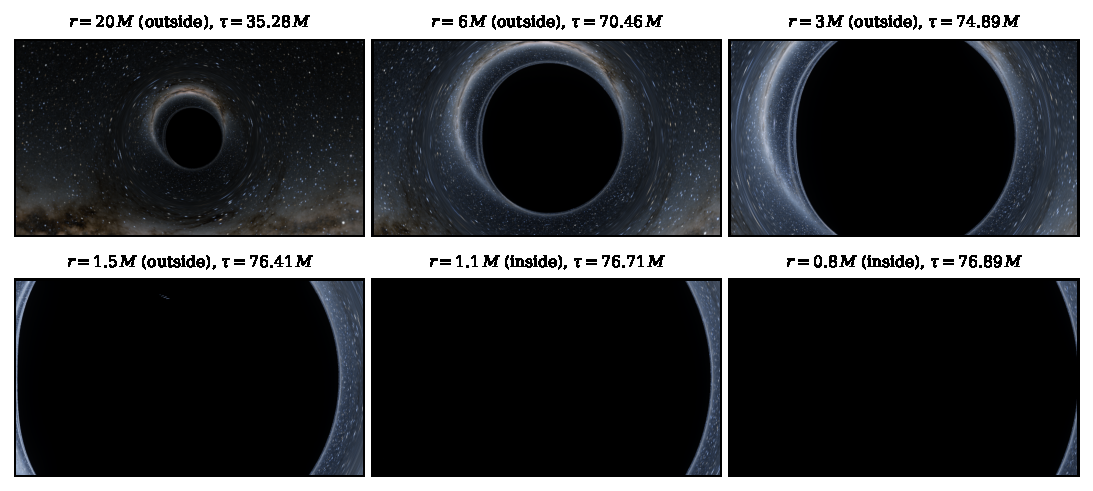
\includegraphics[width=\textwidth]{figures/fig_x_fall.pdf}
\caption{Falling into \sgra{} ($\astar = 0.94$): the view straight ahead of an
observer dropped from rest at infinity, at polar angle $\XIfTheta\degr$, live
GPU renders of the double-precision worldline (field of view 1.6\,rad; the
lensed Milky Way is the only light). Top: outside the horizon
($r_+ = \XIfRplus\,M$); bottom: just outside it and inside it. Labels give
the radius and the faller's proper time since $r_0 = \XIfRzero\,M$.}
\label{fig:xfall}
\end{figure}

\section{Tides}

The tidal field felt by the faller is the electric part of the Riemann tensor
in its own frame, $E_{ij} = R_{i\alpha j\beta} u^\alpha u^\beta$: two free
particles separated by $\xi$ accelerate apart at $-E_{ij}\xi^j$. The simulator
computes it exactly from the analytic metric. The Christoffel symbols come
from complex-step derivatives, and their derivatives from central differences.
It is checked in two ways. In Schwarzschild it reproduces the radial-fall
values $-2M/r^3$ and $M/r^3$, also inside the horizon. And everywhere on the
trip $8(E_{ij}E^{ij} - B_{ij}B^{ij})$ equals the closed-form Kretschmann
scalar of Kerr to $\XIfKretErr$.

\sgra{} is gentle. Across a 2\,m body, the tidal stretch is
$\XIfStretchHor$\,m\,s$^{-2}$ at the horizon and $\XIfStretchEnd$\,m\,s$^{-2}$
at the end of the trip (Fig.~\ref{fig:xfallreadouts}, right). Tides scale as
$M/r^3$, and the horizon radius scales with $M$, so at the horizon they fall
as $1/M^2$. A black hole of four million solar masses can be entered intact;
a stellar-mass one could not be.

\begin{figure}
\centering
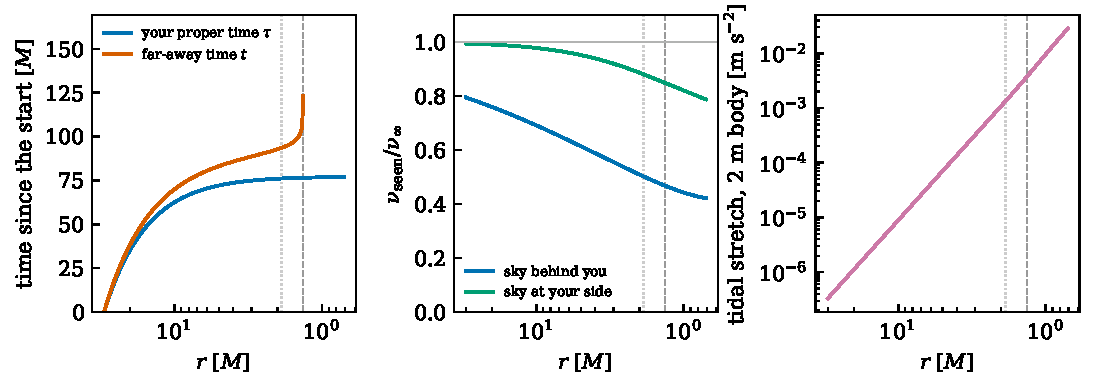
\includegraphics[width=\textwidth]{figures/fig_x_fall_readouts.pdf}
\caption{The faller's instruments along the trip (dashed: the horizon; dotted:
the ergosphere at this latitude). Left: its proper time and the far-away
time, which diverges at $r_+$. Middle: frequency of the sky light arriving
from straight behind and from the side, relative to its frequency at
infinity. Right: tidal stretch across a 2\,m body.}
\label{fig:xfallreadouts}
\end{figure}

\section{Limits}

The fall is classical, vacuum Kerr, along one geodesic. The accretion flow,
the hypothetical disk and every quantum effect are left out, and the trip
stops at the inner horizon by design. The sky is the panorama seen from Earth,
used as the distant background, as in the rest of this report. The camera
frame is one choice among many: another tetrad rotates or boosts the view but
changes no physics.

\chapter{Discussion and Limitations}
\label{ch:xdiscussion}

The chapters so far share a pattern: each new capability is first a
double-precision tool tested against closed forms, then a live rendering
path compared with that tool. The comparisons are what make the images
defensible, and they have found real defects. Three were in the renderer:
the double-counted colour, the step budget and the missing constraint
projection. Two were in the orbit fitting. The forecast Jacobian needs
finite-difference steps far smaller than the thesis used, and the thesis'
direct no-hair fit cannot move $\epsq$ off its starting value
(Chapter~\ref{ch:xforecast}). Several limitations remain and are stated
where they arise.

\begin{itemize}
\item \emph{The thin disk is hypothetical.} At \sgra's measured accretion
rate a thin, radiatively efficient disk would be $\XLumFactorLow$--$\XLumFactorHigh$
times too luminous (\S\ref{sec:thindisk}). The renders that show one are
labelled as such; the physical flow is the subject of
Chapter~\ref{ch:xriaf}.
\item \emph{The sky is Earth's.} The Milky Way panorama is the sky seen from
the Solar System, used as a backdrop at infinity, and its colour shift treats
each pixel as a 6500\,K blackbody (\S\ref{sec:sky}).
\item \emph{The hot spot is the simplest model.} A rigid Gaussian on a
circular geodesic, optically thin, with a fixed spectral index. It
reproduces the GRAVITY periods and sense of rotation but not the size of the
observed centroid motion, exactly the tension GRAVITY reported. Shear, cooling,
out-of-plane motion and polarisation are not modelled
(Chapter~\ref{ch:xflares}).
\item \emph{Display processing is not physics.} Bloom, tone curves, white
balance and false colour are confined to the display chain and are switched
off in every quantitative comparison (\S\ref{sec:display}).
\item \emph{The accretion flow is a semi-analytic RIAF, not a simulation.}
Its radial profiles are fixed power laws, its electrons are purely thermal,
and its one free parameter is fitted to a single flux density. The
comparison with the EHT ring is therefore a test of this family of models,
not of general relativity. In that test the family's reference temperature
fails: the ring is too small. The thesis' critical-curve metrology, which
needs no emission model, remains the result that tests the spacetime.
\item \emph{Polarisation without Faraday effects.} Rotation and conversion in
the flow are omitted, and the intrinsic polarisation fraction is a fixed
assumption. Only quantities independent of that fraction --- the phase of
$\beta_2$ and $|\beta_2|/|\beta_1|$ --- are compared with the EHT. Interstellar
scattering toward \sgra{} is not modelled; the EHT notes that it barely
affects $\beta_2$ \citep{EHT2024pol}.
\end{itemize}

\begin{itemize}
\item \emph{The forecasts are idealised.} They use noise-free data, sampled
uniformly with no seasonal gaps, and include no reference-frame systematics,
source confusion or second star. They are local (Fisher) estimates, checked
against full profile-likelihood fits to within $\XFcProfAgree$ per cent. The
extended mass is a single Plummer profile at GRAVITY's scale radius, and the
spin axis lies along the line of sight. Both choices change the numbers,
though not the conclusion that an extended mass must be fitted with any
future no-hair or spin test (Chapter~\ref{ch:xforecast}).
\item \emph{The wormhole is not \sgra.} The Dneg metric is a test of the
renderer's generality. The exotic matter it would need is not modelled, its
other universe's sky is an illustrative recolouring, and nothing about the
existence of such objects is implied (Appendix~\ref{app:xwormhole}).
\item \emph{The fall is classical and stops at $r_-$.} It is one geodesic in
vacuum Kerr: no accretion flow, no quantum effects, and no interior beyond
the inner horizon, where mass inflation makes the classical solution
unreliable (Chapter~\ref{ch:xinfall}).
\end{itemize}

\chapter{Conclusions}
\label{ch:xconclusions}

The simulator now shows \sgra{} as an observer would see it and keeps the
thesis' standard of evidence. The main results so far:
\begin{itemize}
\item A thin disk fed at the measured accretion rate would be a blue-white
disk at $\XTpeakLow$--$\XTpeakHigh$\,K, and $\XLumFactorLow$--$\XLumFactorHigh$
times brighter than \sgra{} is: the accretion flow must be radiatively
inefficient.
\item A moving observer's view follows from a Lorentz-boosted tetrad alone,
and is verified against Synge's shadow plus aberration to
$\XAberrationCheck$ and in the live renderer to $\XObsGpuMaxPx$ pixel.
\item On the orbits GRAVITY fitted to the 2018 flares, a hot spot traced with
slow light reproduces the period and clockwise sense of the observed loops,
moves only half as far as observed in 30 minutes, and echoes every flash
$\XFlGraEchoMinMin$--$\XFlGraEchoMaxMin$ minutes later in its lensed image.
\item A radiatively inefficient flow normalised to the EHT's
$\XRiafTarget$\,Jy puts its 230\,GHz light in a crescent inside the photon
ring. Its ring is $\XRiafRingDeficit$ per cent smaller than the EHT's unless
its electrons are cooler. Its polarisation reproduces the EHT's spiral only
with a vertical, poloidal magnetic field.
\end{itemize}

\begin{itemize}
\item Continued monitoring of S2 tightens the no-hair parameter much faster
than the thesis' $1/\sqrt{N}$ extrapolation: ten more orbits of existing
quality reach $\sigma(\epsq) = \XFcTenFisher$, not $\XFcTenThesis$. An
extended mass at GRAVITY's present bound, if left out of the fit, turns into
a false no-hair signal of $\XFcBiasEpsThirtyTwo\sigma$ after 32 years. Fitted
jointly, it costs a factor of only $\XFcInflThirtyTwo$ in $\sigma(\epsq)$.
\item Frame dragging in S2's orbit reaches $3\sigma$ after
$\XFcLtThreeTen$\,yr at $10\,\muas$ astrometry, and after
$\XFcLtThreeSixtyFive$\,yr at today's $65\,\muas$. With an extended mass
fitted alongside, these become $\XFcLtThreeTenMarg$\,yr and
$\XFcLtThreeSixtyFiveMarg$\,yr.
\item The renderer is not tied to Kerr. On the Interstellar wormhole, its live
image reproduces the exact edge of the other universe within $\XWhGpuMaxPx$
pixel.
\item Falling into \sgra{} from $\XIfRzero\,M$ takes $\XIfTauHorMin$ minutes
of the faller's time to the horizon and $\XIfTauInsideSec$\,s more to the
inner horizon. It is gentle: the tidal stretch across a 2\,m body is
$\XIfStretchHor$\,m\,s$^{-2}$ at the horizon. The live view is checked
against the double-precision tracer, inside the horizon as well as outside,
to within $\XIfGpuMaxPx$ pixels.
\end{itemize}


\appendix
\chapter{An Exotic Spacetime: the Traversable Wormhole}
\label{app:xwormhole}

\emph{Nothing in this appendix describes \sgra.} It applies the simulator to
a hypothetical spacetime, the Double Negative (``Dneg'') wormhole designed for
the film \emph{Interstellar} by \citet{James2015wormhole} after the
traversable wormholes of \citet{MorrisThorne1988}. The point is to test the
code's generality: the same camera, sky and validation machinery, applied to a
metric that is not Kerr. In the simulator it is reached only through a
separate menu entry, \textsc{exotic (not sgr a*)}. A banner on screen says the
same, and none of its numbers enter any \sgra{} result.

\section{The metric and its rays}

The Dneg wormhole without gravity \citep[][eqs.~1 and 5]{James2015wormhole}
is
\begin{equation}
ds^2 = -dt^2 + d\ell^2 + r(\ell)^2\,(d\theta^2 + \sin^2\theta\,d\phi^2),
\label{eq:dneg}
\end{equation}
\begin{equation}
r(\ell) = \begin{cases}
\rho & |\ell| \le a, \\[2pt]
\rho + M\left[x \arctan x - \tfrac12 \ln(1 + x^2)\right],
\quad x = \dfrac{2(|\ell| - a)}{\pi M} & |\ell| > a .
\end{cases}
\end{equation}
The proper radial distance $\ell$ runs from $-\infty$ (the other universe)
through the cylindrical throat of radius $\rho$ and length $2a$ to $+\infty$
(our universe). The parameter $M$ sets how gently the mouths flare out.
\citet{James2015wormhole} describe the flare by the \emph{lensing width}
$W = 1.42953\,M$. It is the lateral distance in the embedding diagram over
which the surface turns from vertical to $45\degr$, which is where
$dr/d\ell = 1/\sqrt2$. Our code finds that point by bisection and reproduces
their coefficient: the numerical $W$ and the closed form agree to
$\XWhWdiff$. We use the film's wormhole throughout, as chosen by Christopher
Nolan \citep{James2015wormhole}: $2a = \XWhA\,\rho$ and $W = \XWhW\,\rho$
($M = \XWhM\,\rho$). The weak Newtonian potential that \citet{James2015wormhole}
added for the spacecraft's trajectory, $|\Phi| \lesssim 10^{-12}$, is
neglected for light, as in their own ray tracing.

With $p_t = -1$ the affine parameter is the time $t$. Two quantities are
conserved: $b = p_\phi$, and the total impact parameter $B^2 = p_\theta^2 +
b^2/\sin^2\theta$. The rays obey their equations (A.7):
\begin{equation}
\frac{d\ell}{dt} = p_\ell, \quad
\frac{d\theta}{dt} = \frac{p_\theta}{r^2}, \quad
\frac{d\phi}{dt} = \frac{b}{r^2\sin^2\theta}, \quad
\frac{dp_\ell}{dt} = B^2\,\frac{dr/d\ell}{r^3}, \quad
\frac{dp_\theta}{dt} = \frac{b^2\cos\theta}{r^2\sin^3\theta} .
\label{eq:dnegrays}
\end{equation}
The fp64 reference (\texttt{science/wormhole}) integrates
eq.~\eqref{eq:dnegrays} backward from the camera with an adaptive
Dormand--Prince scheme (tolerance $10^{-12}$). The camera uses their local
basis $e_x = e_{\hat\ell}$, $e_y = e_{\hat\phi}$, $e_z = -e_{\hat\theta}$. Along
every traced ray $|\Delta B^2|/B^2 \le \XWhMaxdB$ and the null condition
$|p_\ell^2 + B^2/r^2 - 1| \le \XWhMaxH$.

The live renderer uses the fact that, by spherical symmetry, each ray moves in
a plane through the centre (its lateral motion follows a great circle;
\citealp{James2015wormhole}). It therefore integrates the planar form
$d\ell/dt = p_\ell$, $d\psi/dt = B/r^2$, $dp_\ell/dt = B^2 r'/r^3$ in fp32 RK4.
Here $\psi$ is the angle swept from the camera's position, and the polar
singularity of eq.~\eqref{eq:dnegrays} never arises. Both integrations stop
once the ray is far out and receding ($|\ell| \ge 400\,\rho$ on the CPU,
$40\,\rho$ on the GPU). The remaining sweep, $\arcsin(B/r)$, is then added as
a straight line. Out there $dr/d\ell = 1 - O(M/\ell)$, so that completion errs
by $O(BM/\ell^2)$: moving the CPU stopping point from $400\,\rho$ to
$4000\,\rho$ shifts the Einstein rings below by at most
$\XWhRingShift$\,degrees.

\section{The edge of the other universe}

The radial equation has an exact first integral, $p_\ell^2 = 1 - B^2/r(\ell)^2$.
Since $r$ is smallest, $r = \rho$, along the whole throat, a ray gets through
if and only if $B < \rho$. A ray leaving the camera at angle $\alpha$ from the
direction of the wormhole has $B = r(\ell_c)\sin\alpha$. The other universe
therefore fills a disk on the camera's sky whose edge is exactly at
\begin{equation}
\sin\alpha_{\rm edge} = \rho / r(\ell_c),
\label{eq:dnegedge}
\end{equation}
whatever $a$ and $M$ are. This is our own elementary result; we use it as an
exact test of both tracers. Bisecting the CPU tracer for the edge reproduces
eq.~\eqref{eq:dnegedge} to $\XWhEdgeErr$\,degrees. The live GPU path is checked
on 2001-pixel strips along both image axes through the centre, using a
validation mask (rays that end in our universe are white, rays that end in the
other universe are black). All four edges (left, right, top, bottom) lie within
$\XWhGpuMaxPx$\,pixels of the CPU value at every camera distance
(Table~\ref{tab:xwormhole}).

Rays with $B$ just above $\rho$ wind around the throat before returning to our
universe, and they image our own sky many times in thin bands around the edge.
In every direction around the wormhole, exactly one of these rays ends at the
point of our celestial sphere directly behind the wormhole. Together they form
the \emph{Einstein ring}, the ring image of a source exactly behind the
wormhole \citep{James2015wormhole}. Its radius on the camera's sky is found by
bisecting for the ray whose final azimuth is $\phi_\infty = \pi$ (the camera
sits at $\phi = 0$).

\begin{table}
\centering
\caption{The Dneg wormhole of \emph{Interstellar} ($2a = \XWhA\,\rho$,
$W = \XWhW\,\rho$) seen from three distances: angular radius of the other
universe (CPU, equal to eq.~\ref{eq:dnegedge}) and of the Einstein ring. The
live GPU edges agree with the CPU edges within $\XWhGpuMaxPx$\,pixels in all
three cases.}
\label{tab:xwormhole}
\begin{tabular}{rrrr}
\toprule
$\ell_c/\rho$ & $r(\ell_c)/\rho$ & edge [deg] & Einstein ring [deg] \\
\midrule
15 & \XWhRFifteen & \XWhEdgeFifteen & \XWhRingFifteen \\
6 & \XWhRSix & \XWhEdgeSix & \XWhRingSix \\
2 & \XWhRTwo & \XWhEdgeTwo & \XWhRingTwo \\
\bottomrule
\end{tabular}
\end{table}

\section{The live demo}

The demo shows our universe as the Milky Way map of Chapter~\ref{ch:xspectral}.
For the other universe, whose sky nobody can know, it shows the same map turned
around with its colour channels swapped, so the dust lanes turn blue and it
cannot be mistaken for ours. This choice is illustrative only and is labelled
as such on screen. Dragging the mouse moves the camera around the wormhole, as
it does around \sgra, and the scroll wheel flies along $\ell$, through the
throat if you keep going. No colour shift is applied, because none exists:
$g_{tt} = -1$ everywhere, so a static camera receives light from either
universe at the frequency it was sent.
Figure~\ref{fig:xwormhole} shows the approach. The sine of the other
universe's angular radius grows as $1/r(\ell_c)$. Around its edge, inside the Einstein ring, lies the strongly
lensed image of our own Milky Way, with the Galactic Centre directly behind the
throat. This is the structure \citet{James2015wormhole} describe for the
film's wormhole. The far universe is seen through the mouth. The star field on
the camera's side forms secondary lensed images near the mouth's edge, which
are very thin for a wormhole this short. The Einstein ring lies just outside
the edge.

\begin{figure}
\centering
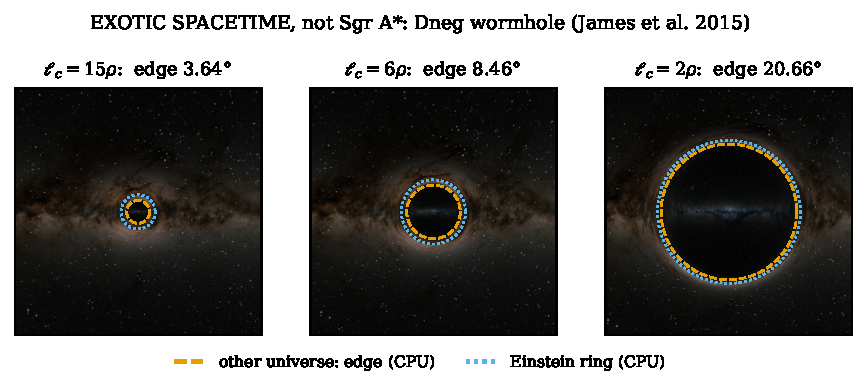
\includegraphics[width=\textwidth]{figures/fig_x_wormhole.pdf}
\caption{\emph{Not \sgra:} the Interstellar wormhole rendered live (GPU),
approached along $\ell$ (field of view 1.2\,rad). The fp64 CPU tracer's
results are overlaid: the edge of the other universe (dashed;
eq.~\ref{eq:dnegedge}) and the Einstein ring (dotted). Inside the edge is the
other universe (an illustrative recoloured sky); outside it is the lensed
Milky Way, with the Galactic Centre behind the throat.}
\label{fig:xwormhole}
\end{figure}

\chapter{Reproducing This Report}
\label{app:xrepro}

\texttt{make reproduce-ext} runs, in order, every tool whose output this
report quotes, then regenerates the numbers and figures:

\begin{center}
\small
\begin{tabular}{p{5.6cm}p{6.6cm}}
\toprule
Command & Produces \\
\midrule
\texttt{ctest --preset sci-rel} & all unit tests (thesis and extension) \\
\texttt{spectral\_tool} & \texttt{spectral.json}: thin disk at the measured $\dot M$; visual vs bolometric contrast \\
\texttt{compare\_live\_colour.py} & \texttt{g13\_colour.json}: live colour vs CPU reference \\
\texttt{observer\_tool} & \texttt{observers.json}: observer kinematics and shadow edges \\
\texttt{compare\_observers.py} & \texttt{g17\_observers\_gpu.json}: live observers vs fp64 \\
\texttt{flare\_tool} & \texttt{flares.json}, light curves, centroid tracks, echoes, images \\
\texttt{compare\_flare.py} & \texttt{g18\_flare\_gpu.json}: live hot spot vs fp64 \\
\texttt{riaf\_tool} & \texttt{riaf.json}: 230\,GHz flow, fit, ring, visibilities, sensitivity, polarisation \\
\texttt{compare\_riaf.py} & \texttt{g19\_riaf\_gpu.json}: live 230\,GHz band vs fp64 \\
\texttt{forecast\_tool} & \texttt{forecasts.json}: Fisher forecasts and extended-mass biases (reads the thesis fit, \texttt{validation/phase5}) \\
\texttt{wormhole\_tool} & \texttt{wormhole.json}: the exotic Dneg wormhole (not \sgra) \\
\texttt{compare\_wormhole.py} & \texttt{wormhole\_gpu.json}: live wormhole edges vs fp64 \\
\texttt{infall\_tool} & \texttt{infall.json}: the fall into \sgra{} (worldline, light, tides, reference strips) \\
\texttt{compare\_infall.py} & \texttt{g24\_infall\_gpu.json}: live in-fall view vs fp64, continuity through $r_+$ \\
\texttt{render\_ext\_gallery.py} & engine renders used as figures \\
\texttt{make\_flare\_movie.py} & one-orbit flare movie (GIF) \\
\texttt{make\_numbers\_ext.py} & \texttt{numbers\_ext.tex}, \texttt{tab\_*.tex} \\
\texttt{make\_figures\_ext.py} & \texttt{figures/} \\
\bottomrule
\end{tabular}
\end{center}

\noindent Tools write to \texttt{validation/extension/}; the GPU comparisons
need the Vulkan build (\texttt{cmake --build --preset engine-rel}) and run
with the validation layers on, which must report zero errors.


\bibliographystyle{mnras}
\bibliography{../refs,refs_ext}

\end{document}
